\chapter{Principe de la tomographie}
	\label{chap:1}
	\graphicspath{{Chap1/}}
	
\vfill
\begin{center}
\includegraphics[scale=0.35]{AdobeStock_109690677.png}
\end{center}
\vfill
{\hypersetup{linkcolor=black}
\minitoc}    % The table of content of the chapter
\vfill
\newpage

Le but de ce chapitre est de donner le contexte physique de la reconstruction tomographique en imagerie dentaire. Nous allons tout d'abord expliquer les fondements de la radiographie, qui constitue la base de la tomographie par rayons X. Pour cela, nous allons suivre le cheminement des rayons X, de leur création jusqu'à leur arrivée sur le détecteur en passant par la traversée du patient. Nous expliquerons comment les interactions entre les rayons et la matière permettent d'obtenir une image de l'intérieur du patient. Nous verrons ensuite comment ont évolué les scanners au fil du temps et les différentes géométries qu'ils utilisent. Enfin, nous parlerons des diverses applications en imagerie médicale, et plus particulièrement en imagerie dentaire. Les informations données dans ce chapitre s'appuient principalement sur les livres \citepp{Buzug2011} et \citepp{Hsieh2009}.{\let\thefootnote\relax\footnotetext{Image de couverture~: radiographie d'un gerbera, licence standard obtenue sur Adobe Stock.}}


%********************************************
\section{Aspects physiques de la radiographie}
%********************************************

La radiographie est une technique d'imagerie qui utilise des rayons X (en imagerie médicale), ou gamma (pour les applications industrielles). Ces rayons, extrêmement pénétrants, traversent le patient ou l'objet, et les rayons transmis permettent d'obtenir une image de l'intérieur du volume considéré.

Les rayons X sont un rayonnement électromagnétique similaire à la lumière visible mais de longueur d'onde bien plus faible, allant de quelques picomètres à quelques nanomètres. Contrairement aux rayons lumineux qui sont réfléchis par les objets, les rayons X passent au travers de la plupart des matériaux et sont invisibles à l'\oe il nu. 
En 1895, le physicien Wilhelm Röntgen découvre par hasard des rayons émanant d'un tube de verre qui apparaissent sur du papier photographique. Par leur caractère inconnu, il nomme ces rayons les rayons X. La \fref{fig:OEM} illustre la position des rayons X dans le spectre électromagnétique. Entre 0.01~nm et 0.1~nm ce sont les rayons X dits "durs", utilisés en radiographie médicale ; au dessus de 0.1~nm, ce sont des rayons "mous" moins pénétrants.

Le lien entre longueur d'onde et énergie est donné par la formule :
$$E = h\nu = \frac{hc}{\lambda}$$
avec $h=6.63\times 10^{-34}$~J.s la constante de Planck, $c=3\times 10^{8}$~m.s$^{-1}$ la vitesse de la lumière dans le vide et $\lambda$ la longueur d'onde. Ainsi, les rayons X ont une énergie comprise entre une centaine d'eV à plusieurs MeV.

\begin{figure}[!t]
	\centering
	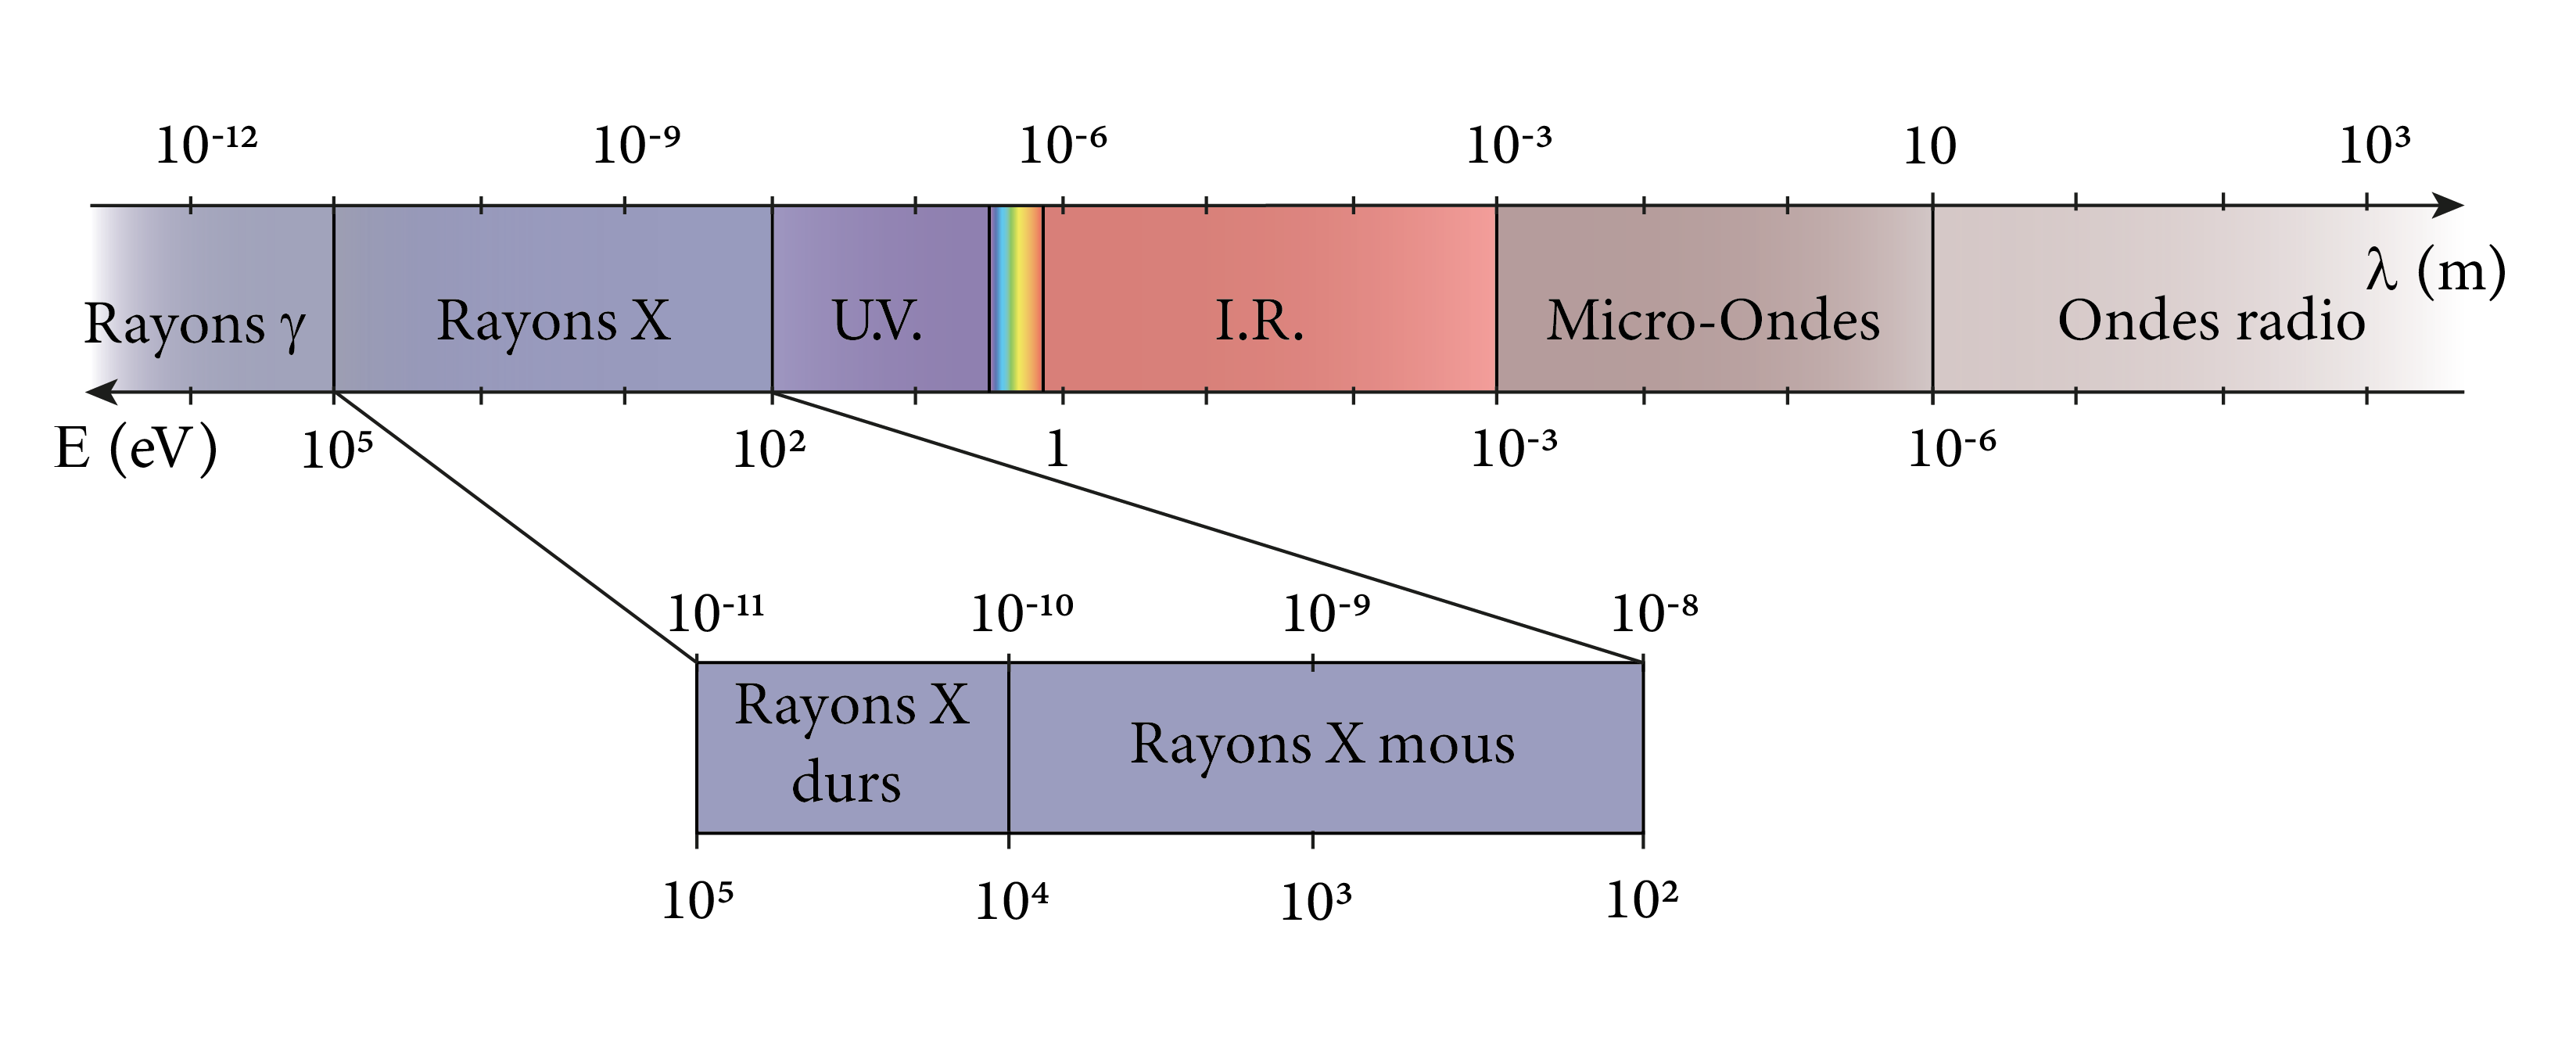
\includegraphics[scale=0.5]{spectre_electromagnetique.png}
	\caption{Spectre électromagnétique.}
	\label{fig:OEM}
\end{figure}

La radiographie utilise le fait que les rayons X peuvent traverser la matière. Ils sont absorbés de manière différente selon le matériau rencontré. Ainsi, les matériaux à forte densité absorbent plus les rayons X que ceux à faible densité. C'est cette propriété qui est utilisée en médecine et qui permet, par exemple, de mettre en évidence les os par rapport au reste du corps humain lors d'une radiographie. La \fref{fig:flower_xray} montre les radiographies d'une fleur et d'une main.

\begin{figure}[!htp]
	\begin{minipage}{0.55\textwidth}
	\centering 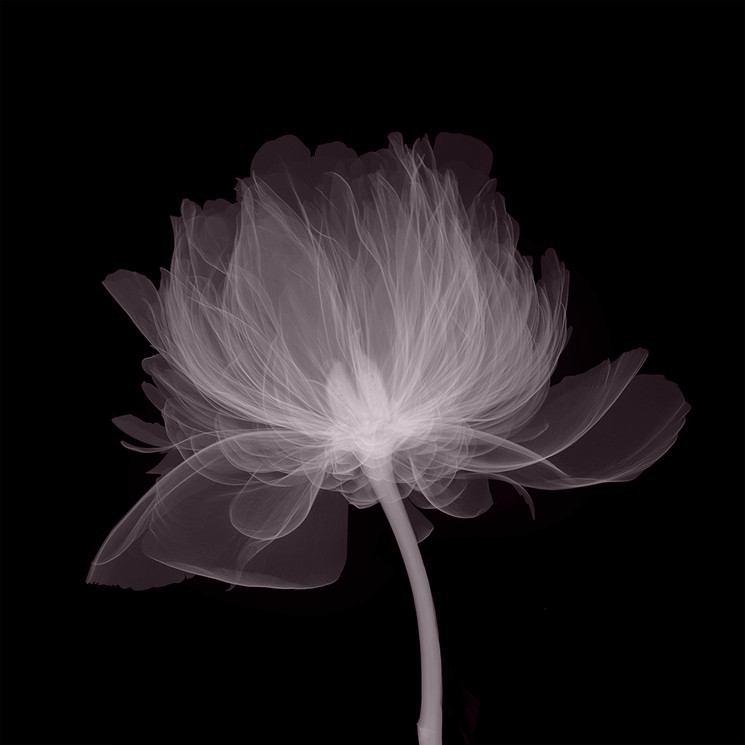
\includegraphics[height=6cm]{Veasey/veasey_flower2_pink.png}
	\end{minipage}
	\begin{minipage}{0.44\textwidth}
	\centering 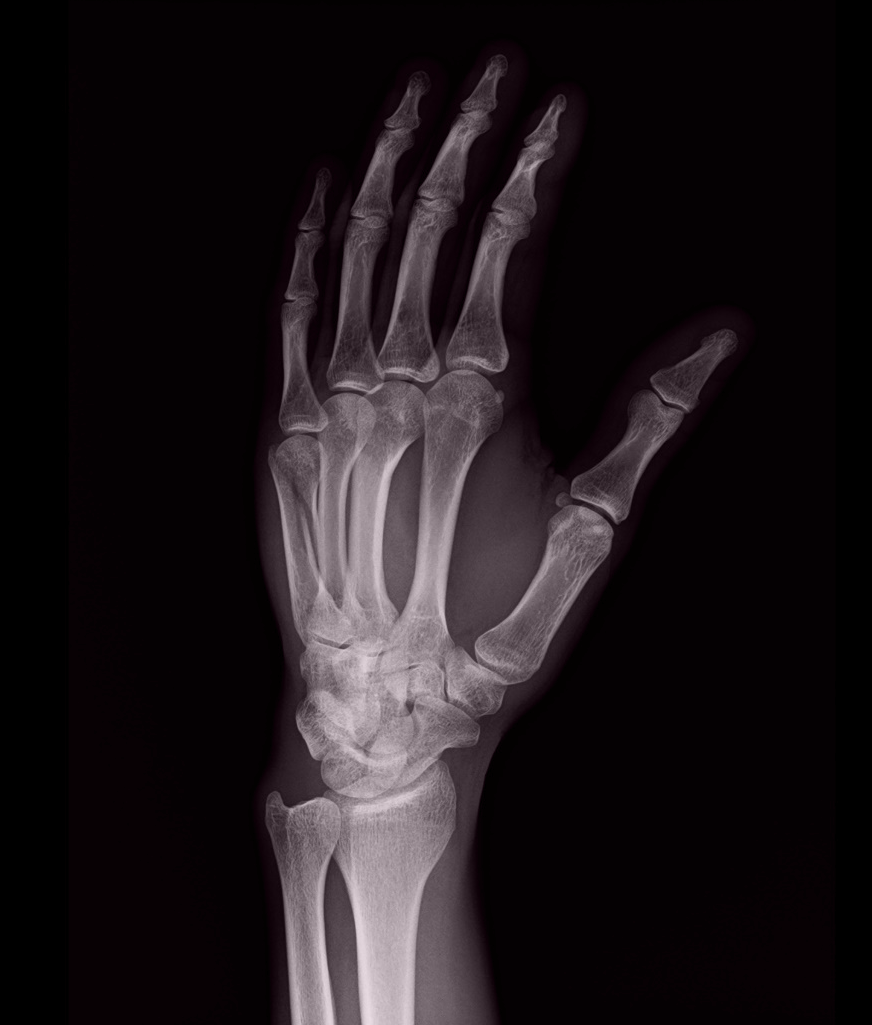
\includegraphics[height=6cm]{Frank1bis.png}
	\end{minipage}
	\caption{Radiographies d'une pivoine\textsuperscript{1} et de la main de Frank Nicolet et sa fracture du cinquième métacarpe après une chute à vélo\textsuperscript{2}.}
\raggedright\footnotesize\textcolor{colorthesis}{\textsuperscript{1}Avec l'autorisation de l'auteur \textcopyright\ Nick Veasey et \textsuperscript{2} autorisation de Frank Nicolet.}
	\label{fig:flower_xray}
\end{figure}

Les rayons X sont utilisés par les radiologues mais également par les dentistes car les os et les dents sont bien contrastés sur la radiographie. On les retrouve également dans les aéroports pour vérifier les bagages, et en archéologie pour révéler des couches dissimulées dans les peintures ou les manuscrits. Les astrophysiciens les utilisent pour étudier la composition des étoiles.

En médecine, l'arrivée des rayons X a été une grande avancée pour l'imagerie médicale. Grâce à eux, les médecins ont pu observer l'intérieur des patients de manière rapide, et sans intervention chirurgicale. 


%----------------------------
\subsection{Tube de Coolidge}

Les rayons X sont principalement produits dans un tube de Coolidge. Il s'agit d'un tube en verre dans lequel se trouvent deux électrodes : une cathode et une anode.

La cathode produit un champ d'électrons qui sont envoyés sur l'anode afin de créer le faisceau de rayons X. Ces deux électrodes sont placées dans une chambre vide en verre pour limiter les interactions avec l'air. 
Les rayons X étant ionisants, il est important d'ajouter une protection autour de la cage en verre pour protéger les opérateurs et les patients des radiations. On utilise une protection en plomb : grâce à son numéro atomique élevé, elle empêche les rayons X de quitter le tube.
Enfin, à la sortie du tube se trouve une plaque en aluminium dont le but est de filtrer les rayons X de basses énergies. Un schéma de ce tube est visible dans la \fref{fig:coolidge}.

\begin{figure}
\centering
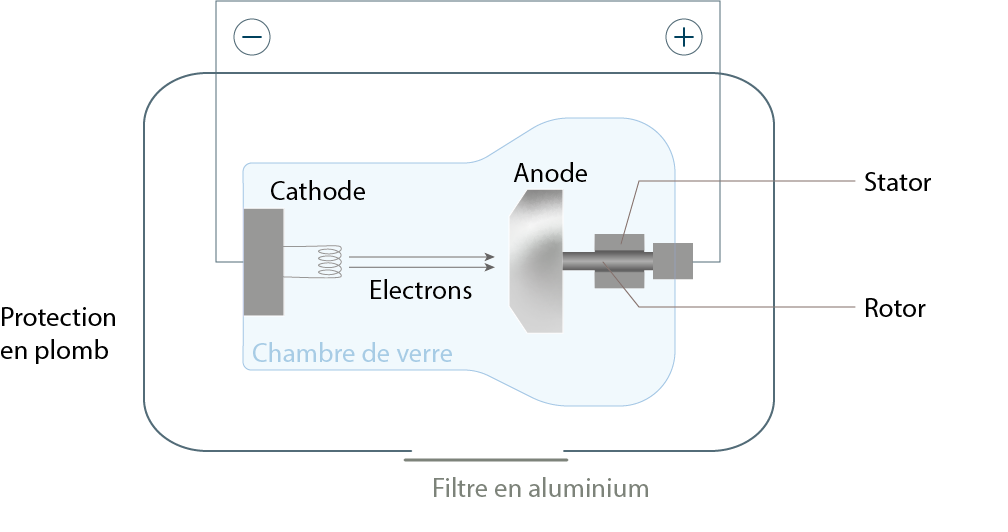
\includegraphics[width=0.7\textwidth,trim = 0cm 0cm 3cm 0cm]{tube_coolidge.png}
\caption{Tube de Coolidge}
\label{fig:coolidge}
\end{figure}


%--------------------------------
\subsection{Création des rayons X}

La création des rayons X résulte d'interactions entre particules relevant de la physique quantique. Elle s'effectue en trois étapes. La première consiste en la création d'un nuage électronique par la cathode. Cette dernière est composée d'un filament de métal que l'on fait chauffer par effet Joule. Le filament se réchauffe et la chaleur provoque une agitation des électrons superficiels dont une partie se détache pour constituer un nuage électronique, c'est le processus d'émission thermo-ionique. L'intensité du faisceau d'électrons est proportionnelle à l'intensité du courant de chauffe de la cathode et à la durée du chauffage.

Pendant la deuxième étape, les électrons arrachés des atomes du filament  sont accélérés et envoyés sur l'anode. L'anode est portée à très haute tension, la différence de potentiel entre l'anode et la cathode crée un champ électrique qui accélère les électrons en direction de l'anode. Plus la différence de potentiel est grande, plus l'énergie cinétique des électrons est grande. La cathode et l'anode sont placées dans une chambre vide en verre afin d'éviter que les électrons ne soient déviés par des molécules d'air.

La troisième étape se produit lorsque les électrons interagissent avec l'anode, c'est à ce moment-là que se créent les rayons X. Une fois arrivés sur l'anode, les électrons sont déviés ou entrent en collision avec les atomes de celle-ci. 
\begin{enumerate}
	\item Dans le premier cas, on parle de rayonnement de freinage ({\it Bremsstrahlung}) : l'électron s'approche d'un atome et à cause de sa charge négative, il est attirée par le noyau d'après la loi électrostatique de Coulomb. Il est dévié de sa trajectoire et subit une décélération. La perte d'énergie cinétique de l'électron conduit à l'émission d'un rayonnement. Plus l'écart d'énergie cinétique de l'électron est grand, plus l'énergie du photon émis sera grande. L'effet Bremsstrahlung crée un spectre continu, aussi appelée "radiation blanche". 
	%Si l'électron entre en collision avec le noyau de l'atome, il perd la totalité de son énergie cinétique et crée un rayonnement dont l'énergie est la plus haute possible.
	%Souvent, l'électron est peu ralenti et le photon a une très faible énergie et correspond à de la chaleur.

	\item Dans le second cas, l'électron incident entre en collision avec un des électrons d'une couche profonde d'un atome et l'éjecte de sa couche, l'atome se retrouve ionisé. Pour rétablir l'équilibre, un électron d'une couche supérieure descend remplacer l'électron éjecté. En changeant de couche, cet électron perd de l'énergie, ce qui aboutit à l'émission d'une radiation caractéristique dont l'énergie dépend des couches de l'atome mises en jeu lors de cette interaction. Les différences d'énergie entre les différentes couches d'un atome sont fixées et caractéristiques de cet atome. Ainsi, ce type d'interaction crée des raies caractéristiques dans le spectre d'émission. 
	
	\item Enfin, l'électron peut directement rentrer en collision avec le noyau d'un atome. Dans cette configuration, l'intégralité de l'énergie de l'électron se transforme en photon selon l'effet Bremsstrahlung. L'énergie du rayon X produit par cette interaction est ainsi maximale, cependant, la probabilité d'une telle collision est très faible.  
\end{enumerate}

Durant ce processus, seule une faible partie de l'énergie incidente est transformée en rayons X, 99\% de cette énergie se dissipe en chaleur. Le rendement énergétique est très faible et proportionnel au numéro atomique de l'anode et à la différence de potentiel entre l'anode et la cathode. Pour maximiser le rendement, il est donc préférable de choisir un matériau de numéro atomique élevé et qui soit capable de résister à la chaleur ; en général l'anode est en tungstène, molybdène ou cuivre.

Le spectre de rayons X est obtenu en additionnant le spectre continu créé par l'effet Bremsstrahlung et les radiations caractéristiques qui forment des pics. Un exemple de spectre est montré dans la \fref{fig:emission_spectrum}. Dans ce spectre continu, on retrouve des photons de basse énergie qui sont absorbés par les tissus mous. Ces rayons augmentent la dose de rayons X envoyée au patient et n'apportent aucune contribution utile \citepp{Webb2003}. Ils sont donc filtrés à l'aide d'une plaque en aluminium qui absorbe uniquement les rayons de faible énergie. 

\begin{figure}
	\centering
	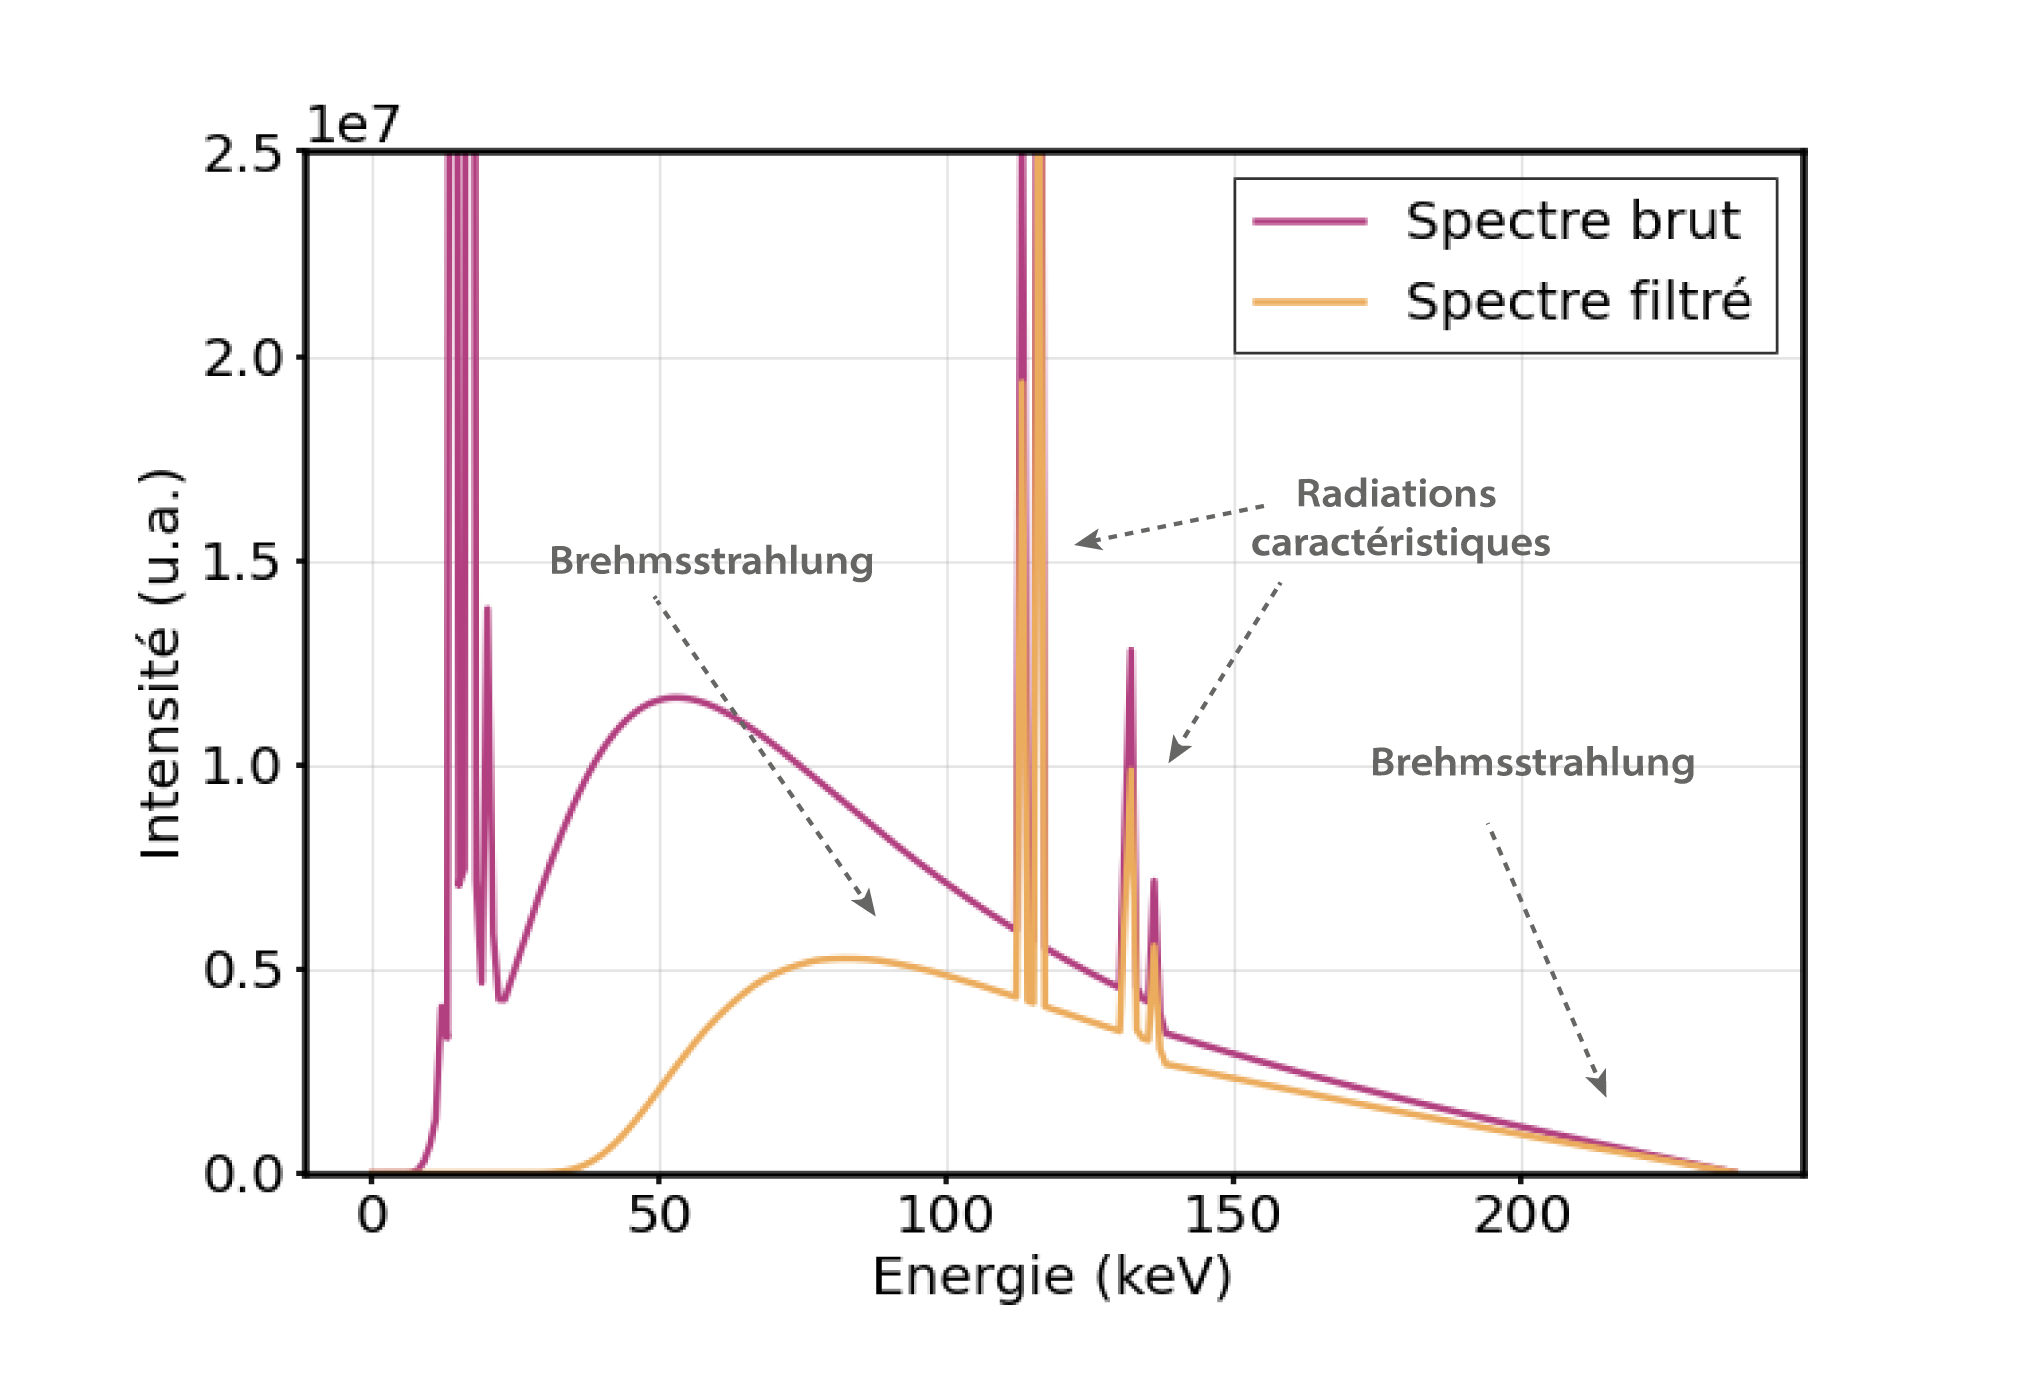
\includegraphics[width=9cm]{emission22-02.png}
	\caption{Spectre de rayons X à la sortie du tube (en rose) et spectre filtré par une plaque d'aluminium d'épaisseur 4~mm (en orange). Simulations faites avec la librairie Spekpy\textsuperscript{1} en Python \citepp{Bujila2020,Poludniowski2021}.}
	\raggedright\footnotesize\textsuperscript{1} \url{https://bitbucket.org/spekpy/spekpy_release/wiki/Home}
	\label{fig:emission_spectrum}
\end{figure} 

Le spectre obtenu est un spectre polychromatique, c'est-à-dire qu'il contient plusieurs longueurs d'onde différentes. En tomographie, nous verrons dans la suite qu'il est préférable de travailler avec des spectres monochromatiques. Un spectre monochromatique pourrait théoriquement être obtenu par filtrage mais au détriment du flux de photons, ce qui compromet son utilisation en médecine. Des faisceaux monochromatiques à fort flux de photons peuvent être obtenus sur des synchrotrons, ce qui permet d'obtenir des images tomographiques quantitatives à fort rapport signal sur bruit, mais cette technique n'est toutefois pas utilisable en imagerie dentaire.


%------------------------------------------
\subsection{Interactions rayons X - matière}
	\label{subsec:inter_x_mat}

Après sa sortie du tube de Coolidge, le faisceau de rayons X traverse le patient, et les rayons non absorbés par le patient forment l'image de radiographie. Durant leur traversée les photons des rayons X interagissent de différentes manières avec la matière. Le type d'interaction dépend de l'énergie des rayons X et des numéros atomiques des atomes rencontrés, on en trouve cinq différents, dont seulement trois dans le domaine d'énergie utilisé en imagerie par rayons X. 
\begin{itemize}
	\item[] {\it Effet photo-électrique}~~~Le photon incident éjecte un électron de l'atome et est complètement absorbé. L'atome se retrouve ionisé et crée un rayonnement caractéristique secondaire pour se stabiliser. C'est l'interaction la plus utile pour la radiographie médicale, elle apparaît pour des énergies entre $10$ et $300$~keV et dépend du numéro atomique de l'atome. Cette dernière propriété est importante : les os, principalement composés de calcium dont le numéro atomique $Z=20$ est supérieur à celui de l'oxygène présent dans l'eau ($Z=8$), absorberont plus les rayons X par effet photo-électrique que les tissus mou. C'est ce qui permettra de distinguer les deux matières sur la radiographie.
	\item[] {\it Effet Compton}~~~Un photon incident de grande énergie entre en collision avec un électron de l'atome mais n'est pas absorbé. L'électron est éjecté et le photon incident, qui a perdu une partie de son énergie, est diffusé dans une direction aléatoire faisant un angle dépendant de l'énergie initiale et de l'énergie perdue. La diffusion Compton est donc aussi appelée diffusion incohérente et elle intervient dans la même plage d'énergie que l'effet photo-électrique. Sa probabilité ne dépend que de la densité électronique du matériau - le nombre d'électrons sur la couche de valence - et non pas du numéro atomique de l'atome. L'absence de lien avec le numéro atomique ne permet pas d'obtenir un bon contraste entre les différents matériaux de densité similaire, et l'angle aléatoire du photon diffusé crée du bruit. Par conséquent, les appareils de tomographie essaient de minimiser l'impact de l'effet Compton, avec une grille par exemple.
	\item[] {\it Diffusion de Rayleigh - diffusion cohérente}~~~Le photon excite l'atome sans collision avec un électron. Le retour à l'état stable de l'atome émet un nouveau photon de même énergie. Cette interaction n'apparaît que lorsque l'énergie du photon est relativement basse et est peu utile en imagerie médicale.
\end{itemize}
Les deux autres interactions, la création de paires ainsi que la photo-désintégration, n'ont lieu que dans des tranches d'énergie très hautes non utilisées en radiographie médicale. La création de paires se produit lorsque le photon interagit au voisinage du noyau de l'atome et qu'un électron et un positon sont créés. Si le photon a une très grande énergie, l'impact de celui-ci avec un atome peut causer la destruction d'une partie du noyau : c'est la photo-désintégration. 

La \fref{fig:inter_matiere} représente les deux principales interactions en radiographie : l'effet photo-électrique et l'effet Compton. Afin de mieux comprendre l'importance relative de chaque interaction, la figure~\ref{fig:percentage_of_interaction} montre le pourcentage d'interaction dans l'eau selon l'énergie du photon. L'effet photo-électrique est prédominant en dessous de 30~keV ; au-delà, l'effet Compton prédomine. La diffusion de Rayleigh a une faible probabilité de se produire pour toutes les énergies. La figure~\ref{fig:percentage_of_transmitted_energy} complète la figure précédente et montre que pour les faibles énergies, la majorité de l'énergie transférée est due à l'effet photo-électrique. 

\begin{figure}
  \begin{center}
    \subfloat[Effet photo-électrique]{
      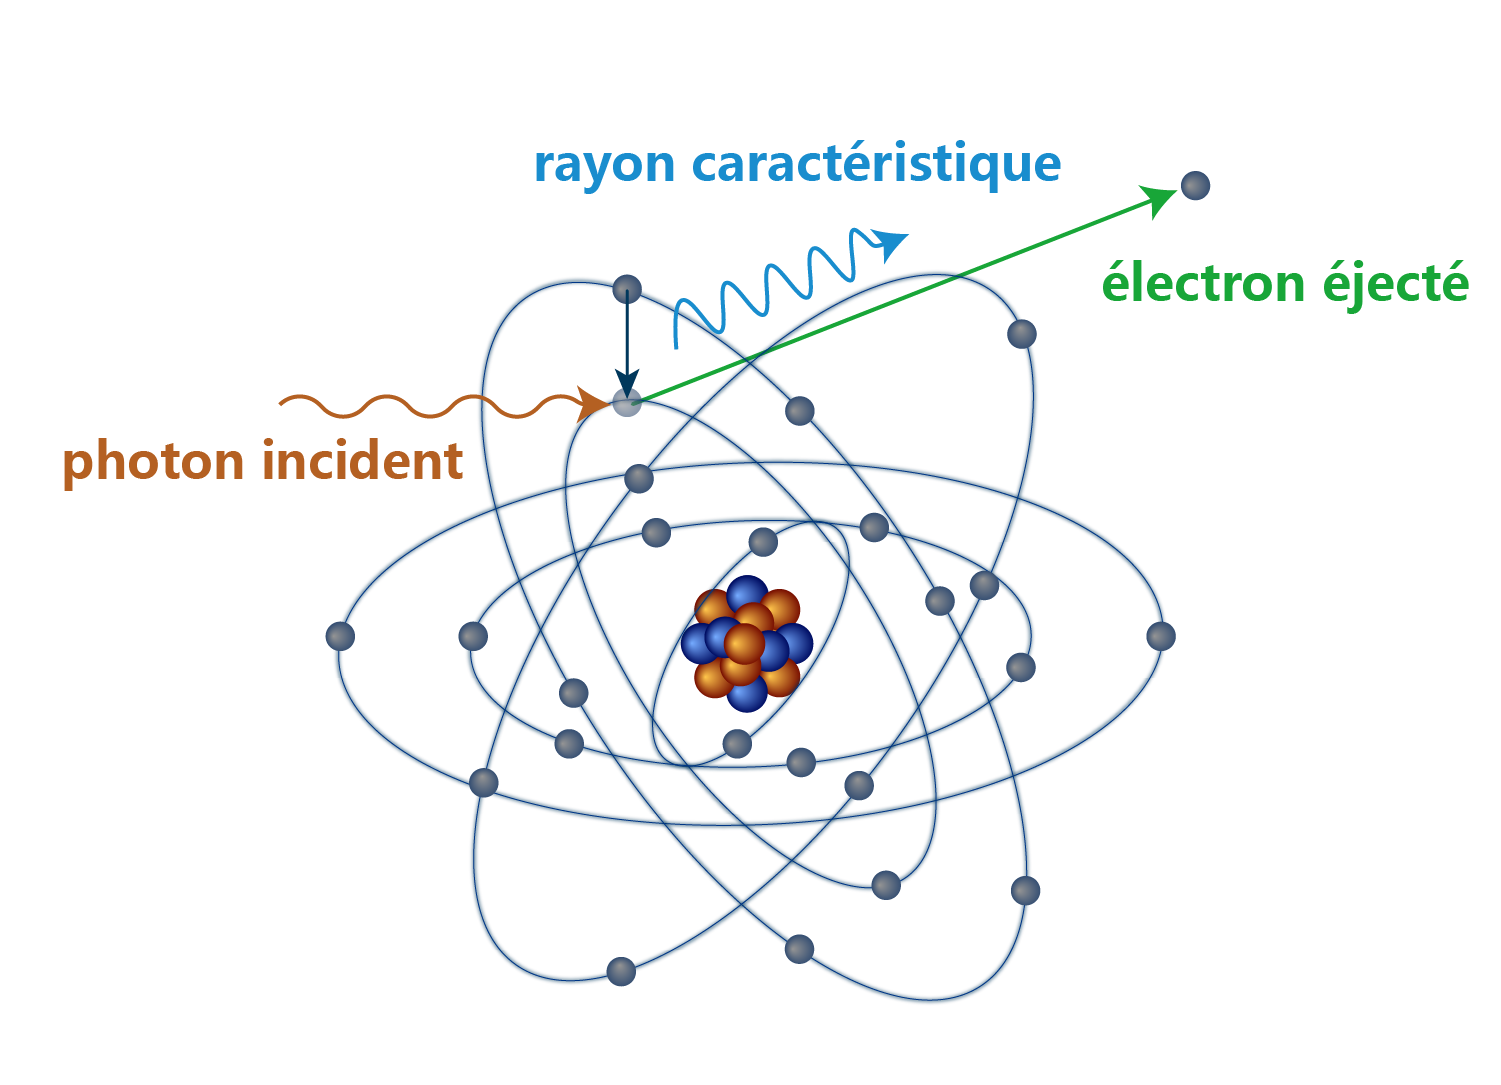
\includegraphics[width=0.4\textwidth]{effet_pe.png}
      \label{sub:effet_pe}
                         }
    \subfloat[Effet Compton]{
      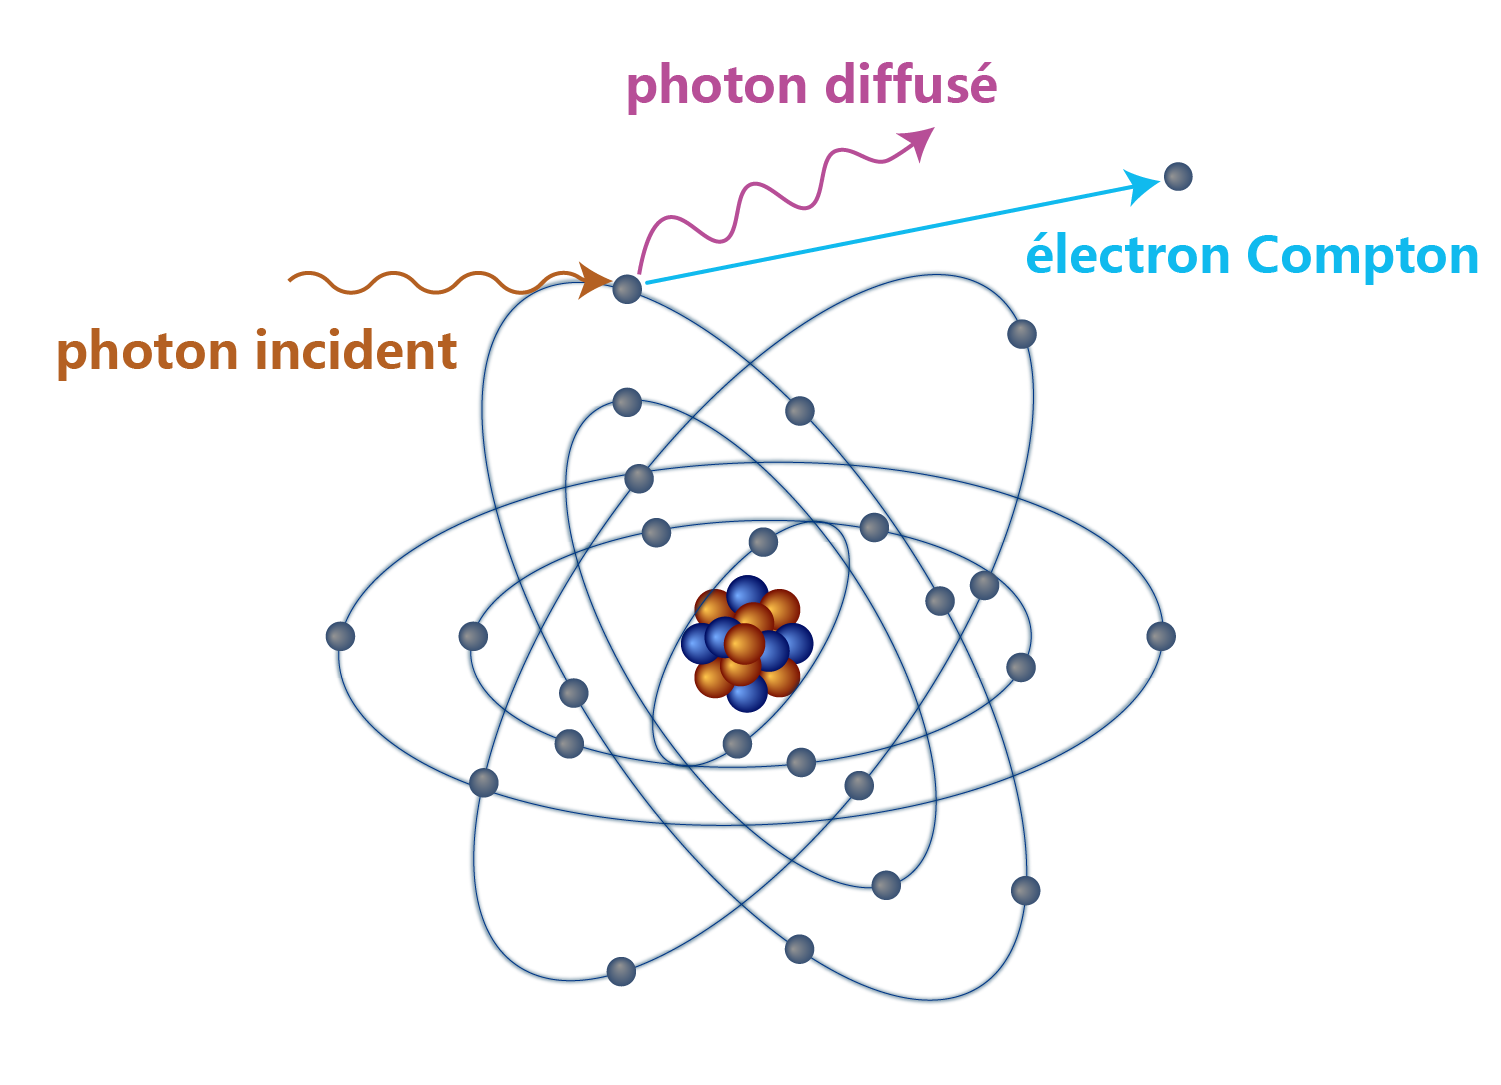
\includegraphics[width=0.4\textwidth]{effet_compton.png}
      \label{sub:effet_compton}
                         }
    \caption{Interactions photon - matière}
    \label{fig:inter_matiere}
  \end{center}
\end{figure}


\begin{figure}
  \begin{center}
    \subfloat[]{
      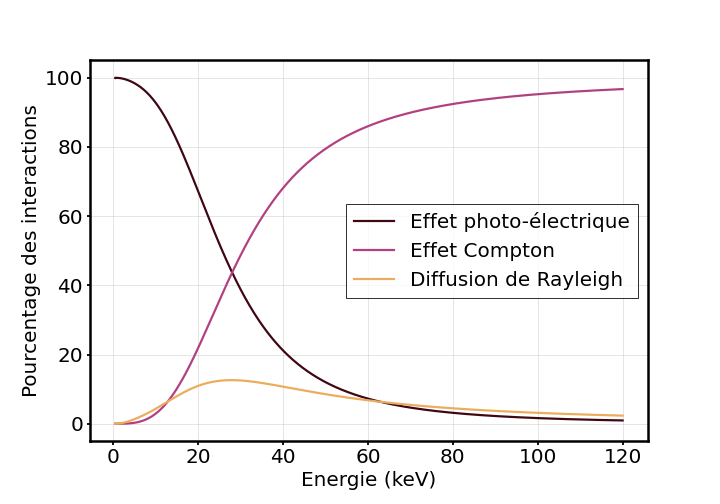
\includegraphics[width=0.46\textwidth,trim=1.2cm 0.8cm 0cm 0cm]{pourcentage_3_effets.png}
      \label{fig:percentage_of_interaction}
                         }
    \subfloat[]{
      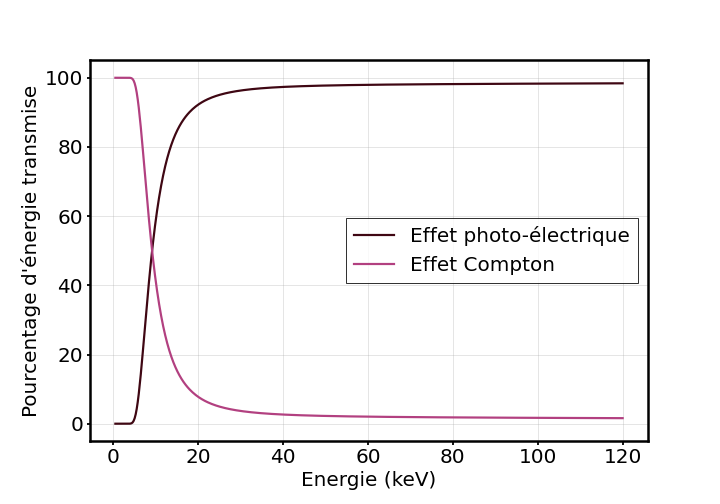
\includegraphics[width=0.46\textwidth,trim=1.2cm 0.8cm 0cm 0cm]{per_nrj.png}
      \label{fig:percentage_of_transmitted_energy}
                         }
    \caption{(a) Pourcentage des trois principales interactions dans l'eau en fonction de l'énergie des rayons X. (b) Pourcentage d'énergie transmise en fonction de l'énergie des rayons X. Simulations effectuées à l'aide de la librairie XrayDB\textsuperscript{1} en Python.}
    \raggedright\footnotesize\textsuperscript{1} \url{https://xraypy.github.io/XrayDB/python.html}
  \end{center}
\end{figure}


D'après ce qui précède, en traversant le patient, les rayons X peuvent être transmis, diffusés ou absorbés. En effectuant une radiographie, nous mesurons l'atténuation que subit le faisceau de rayons X. Le faisceau étant polychromatique (cf figure~\ref{fig:emission_spectrum}), son atténuation vérifie l'équation suivante pour un matériau homogène :
\begin{equation}
	\label{eq:beer-lambert-polychromatique}
	I = \int_0^{E_{\text{max}}} I_0(E)\text{e}^{-\mu(E) L}dE
\end{equation}
avec $I_0$ l'intensité du faisceau X incident, $L$ l'épaisseur du matériau traversé (cm) et $\mu$ le coefficient d'absorption linéaire du matériau (cm$^{-1}$).

En pratique, on suppose le rayonnement monochromatique, l'équation~\textcolor{sub}{(\ref{eq:beer-lambert-polychromatique})} devient :
\begin{equation}
	\label{eq:beer-lambert1}
I = I_0 e^{-\mu L}
\end{equation}
aussi appelée loi d'absorption de Beer-Lambert. 


Ainsi, l'intensité reçue par le détecteur dépend du coefficient d'absorption du matériau. La figure~\ref{fig:linear_coefficient} représente l'évolution du coefficient selon l'énergie pour trois matériaux différents. A partir de 30~keV, l'iode a un coefficient d'absorption beaucoup plus élevé que l'os et l'eau, ce qui en fait un très bon agent de contraste. Il est utilisé pour observer les organes et le sang en angiographie. Le coefficient de l'os est supérieur à celui de l'eau, que l'on identifie aux tissus mous, d'où la nette différence entre le squelette et les tissus sur une radiographie. 

\begin{figure}
	\centering
	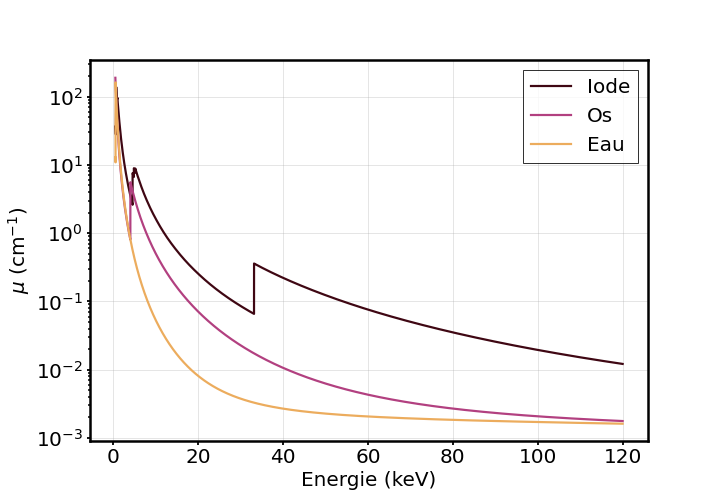
\includegraphics[width=0.45\textwidth]{absorption_mat.png}
	\caption{Coefficient d'atténuation linéaire pour l'iode, les os et l'eau en fonction de l'énergie. Simulations effectuées à l'aide de la librairie XrayDB en Python.}
	\label{fig:linear_coefficient}
\end{figure}


%---------------------------------------------
\subsection{Détection et formation de l'image}

Une fois que les rayons X ont traversé le corps du patient, il faut les quantifier. Au début de la radiographie, on utilisait des films photosensibles avec un fonctionnement similaire à celui de la photographie argentique classique. Des cristaux d'argent présents sur le film sont ionisés lorsqu'ils reçoivent le rayonnement, ils créent des amas d'atomes d'argent qui forment l'image visible. Ainsi, l'image est plus sombre là où elle a reçu plus de rayons, ce qui explique que les tissus mous qui laissent passer plus de rayons ressortent en noir et les os en blanc sur une radiographie. 

Lors de l'apparition des premiers capteurs plans, ces films ont été délaissés au profit de leur version numérique qui permet de faire le traitement des images obtenues par ordinateur. On retrouve deux types de détecteurs, les détecteurs indirects et les détecteurs directs \citepp{Rowlands2002}. 
\begin{itemize}
	\item[] Les {\it détecteurs indirects} sont constitués d'un scintillateur et de photo-diodes. Le scintillateur convertit les rayons X en rayons lumineux. Avec un matériau tel que l'iodure de césium, des photons de fluorescence sont émis par effet photo-électrique dans le domaine du visible. Les photons lumineux sont ensuite transformés en signaux électriques par les photo-diodes. Cependant, lors des interactions dans le scintillateur, certains photons X sont perdus, et les photons lumineux produits n'ont pas nécessairement la même direction que le photon X qui les a produit.
	\item[] Les {\it capteurs directs} détectent les photons X sans transformation préalable et les convertissent directement en signaux électriques. Les photons X sont convertis en paires d'électron-trou dans un semi-conducteur tel que le sélénium amorphe, et les électrons sont collectés pour quantifier le nombre de photon X présents. Par rapport aux détecteurs indirects, ceux-ci ont l'avantage de pouvoir également déterminer l'énergie des rayons X et sont donc utilisés en imagerie spectrale.  De plus, ces capteurs ont une résolution supérieure à celle des capteurs indirects \citepp{Ristic2013}.
\end{itemize}


%*********************************
\section{Géométries d'acquisition}
%*********************************

Comme exposé en introduction, le but de la tomographie est d'observer l'intérieur d'un objet ou d'un patient de manière non invasive à partir de mesures extérieures. En tomographie par rayons X, ces mesures extérieures sont des mesures d'atténuation, prises selon différents angles de vue autour du patient. Au fil des années et des différentes avancées technologiques, les scanners et les techniques d'acquisition ont évolué. Nous présentons ici différentes générations de scanners, que l'on retrouve figure~\ref{fig:scanner_gen} et géométries d'acquisition, figure~\ref{fig:diff_geometry}.

La première géométrie d'acquisition utilisait des rayons X parallèles entre eux : c'est la géométrie parallèle utilisée par les scanners de première génération. Leur but était de reconstruire une coupe, c'est-à-dire une image 2D, de l'intérieur d'un patient. Ils utilisaient un détecteur mono-pixel qui se déplaçait linéairement, en même temps que la source, pour scanner le patient selon un certain angle, ce qui permettait d'obtenir une mesure 1D. Puis l'opération était répétée autant de fois que nécessaire afin d'obtenir les acquisitions sous plusieurs angles (figure~\ref{sub:gen1}). Avec ce type de scanner, le temps d'acquisition était très long (environ 5 minutes) et la qualité des reconstructions diminuée par les mouvements du patient. Cette géométrie n'est aujourd'hui plus utilisée en imagerie médicale.

\begin{figure}[H]
  \begin{center}
    \subfloat[1$^{\text{ère}}$ génération]{
      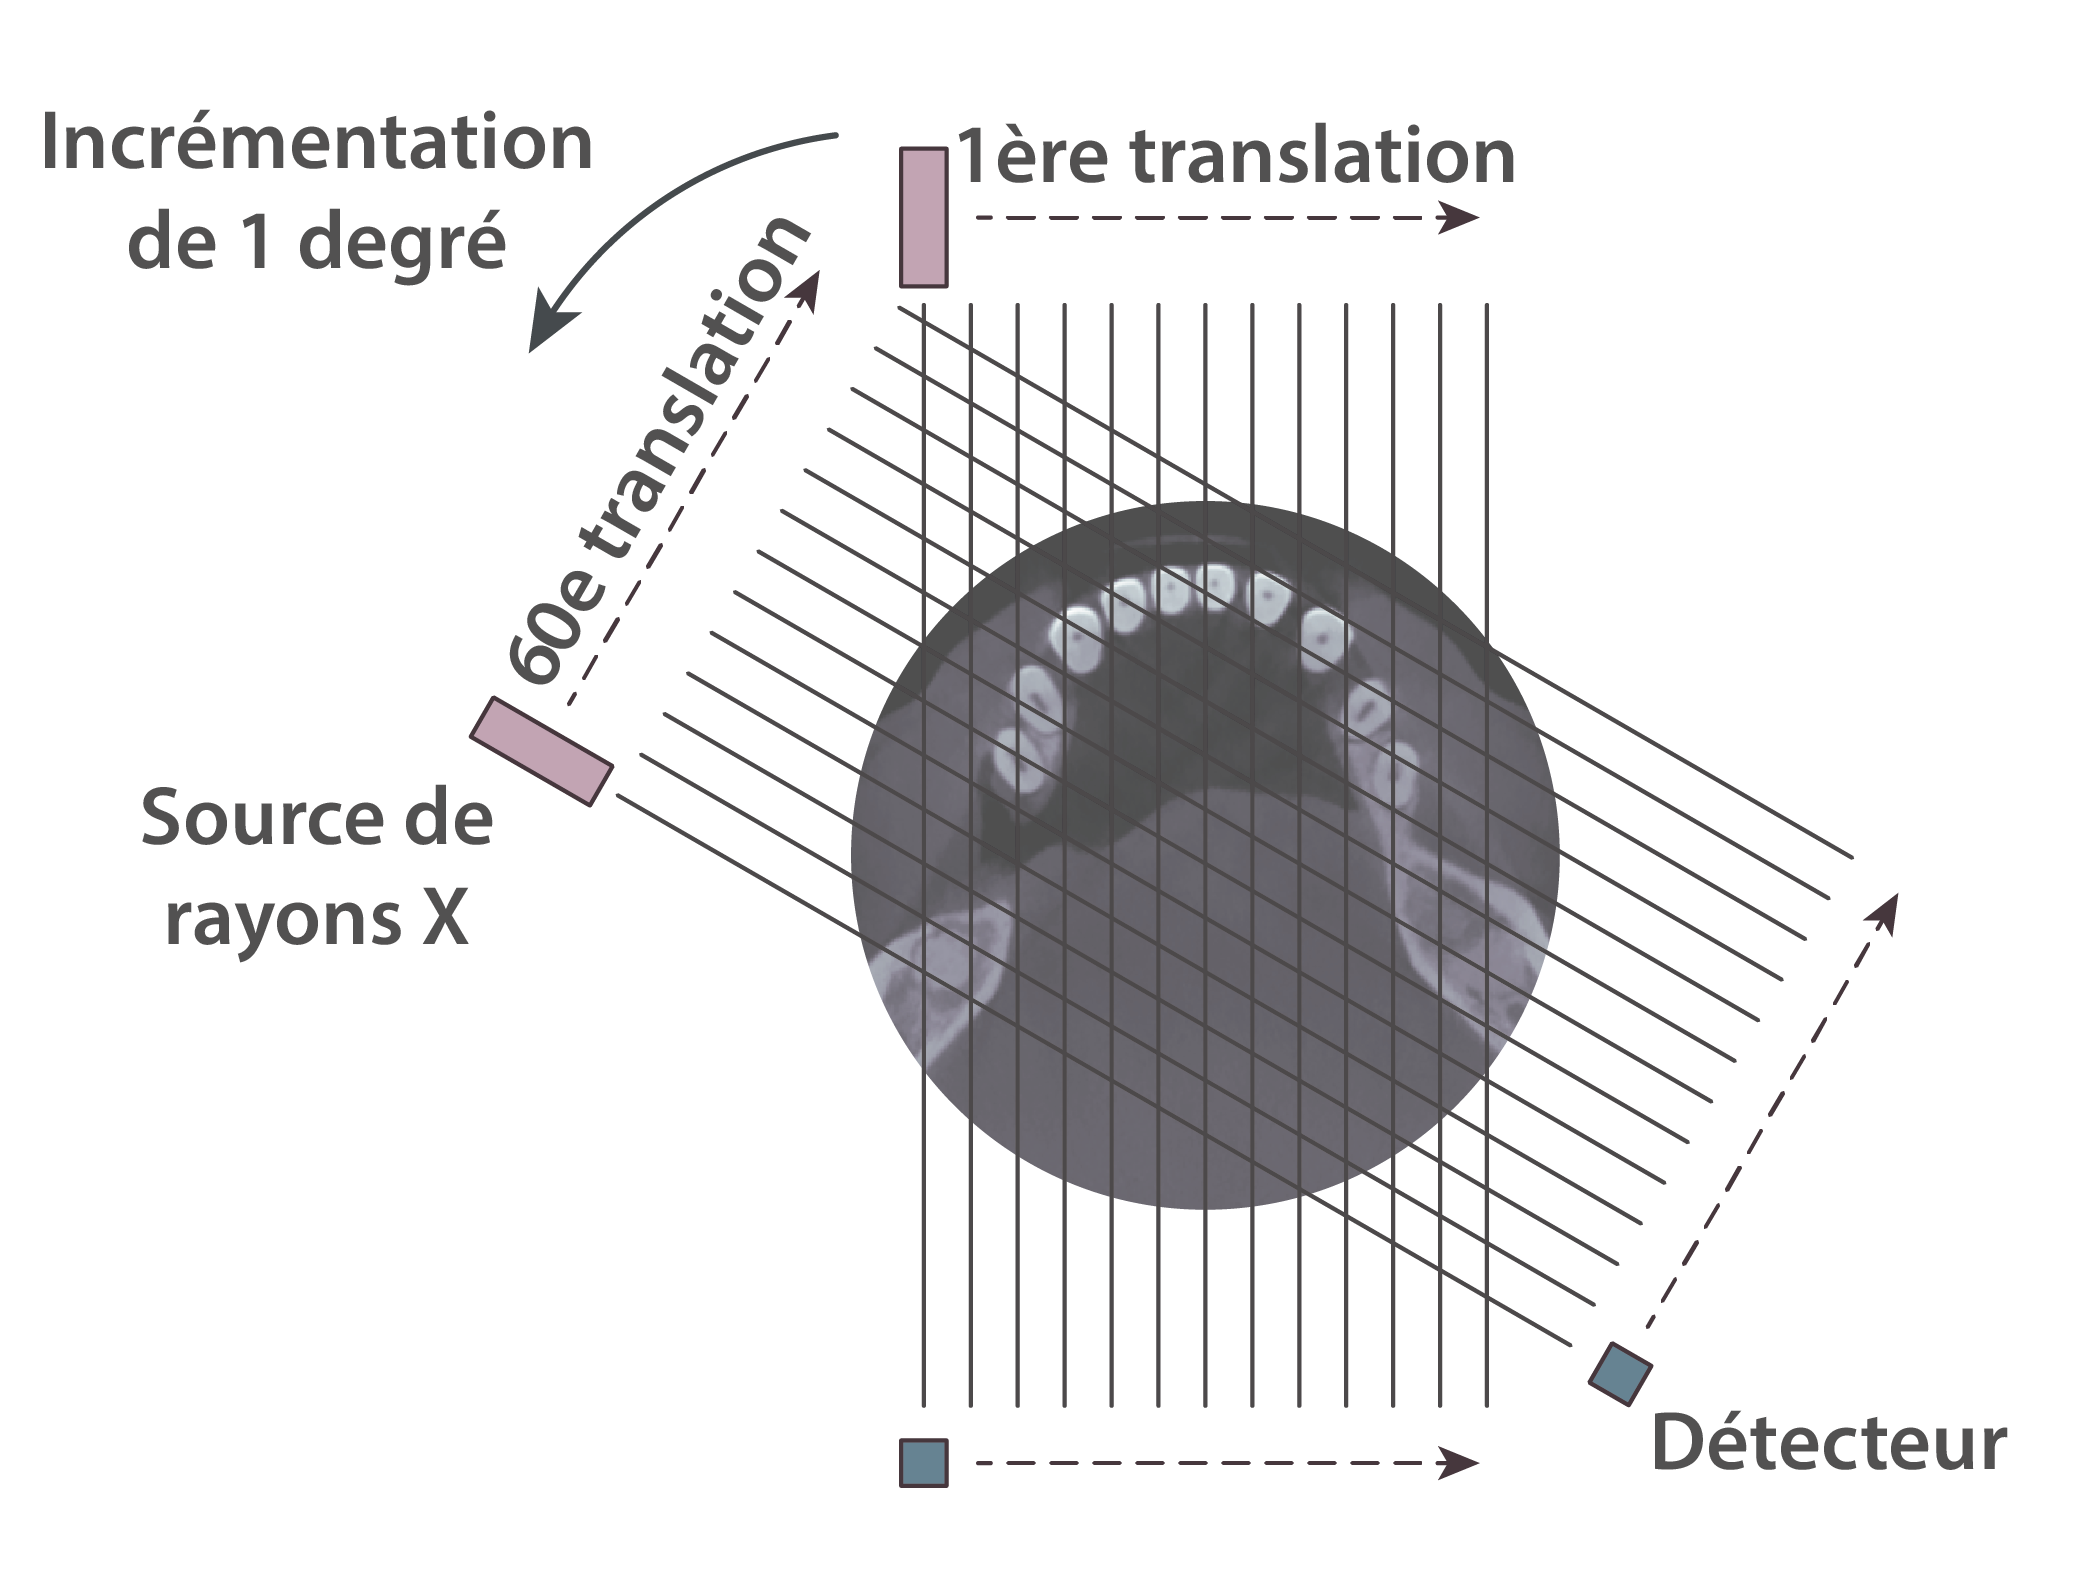
\includegraphics[height=5.5cm]{generation_Generation_1.png}
      \label{sub:gen1}
                         }
    \subfloat[$2^{\text{e}}$ génération]{
      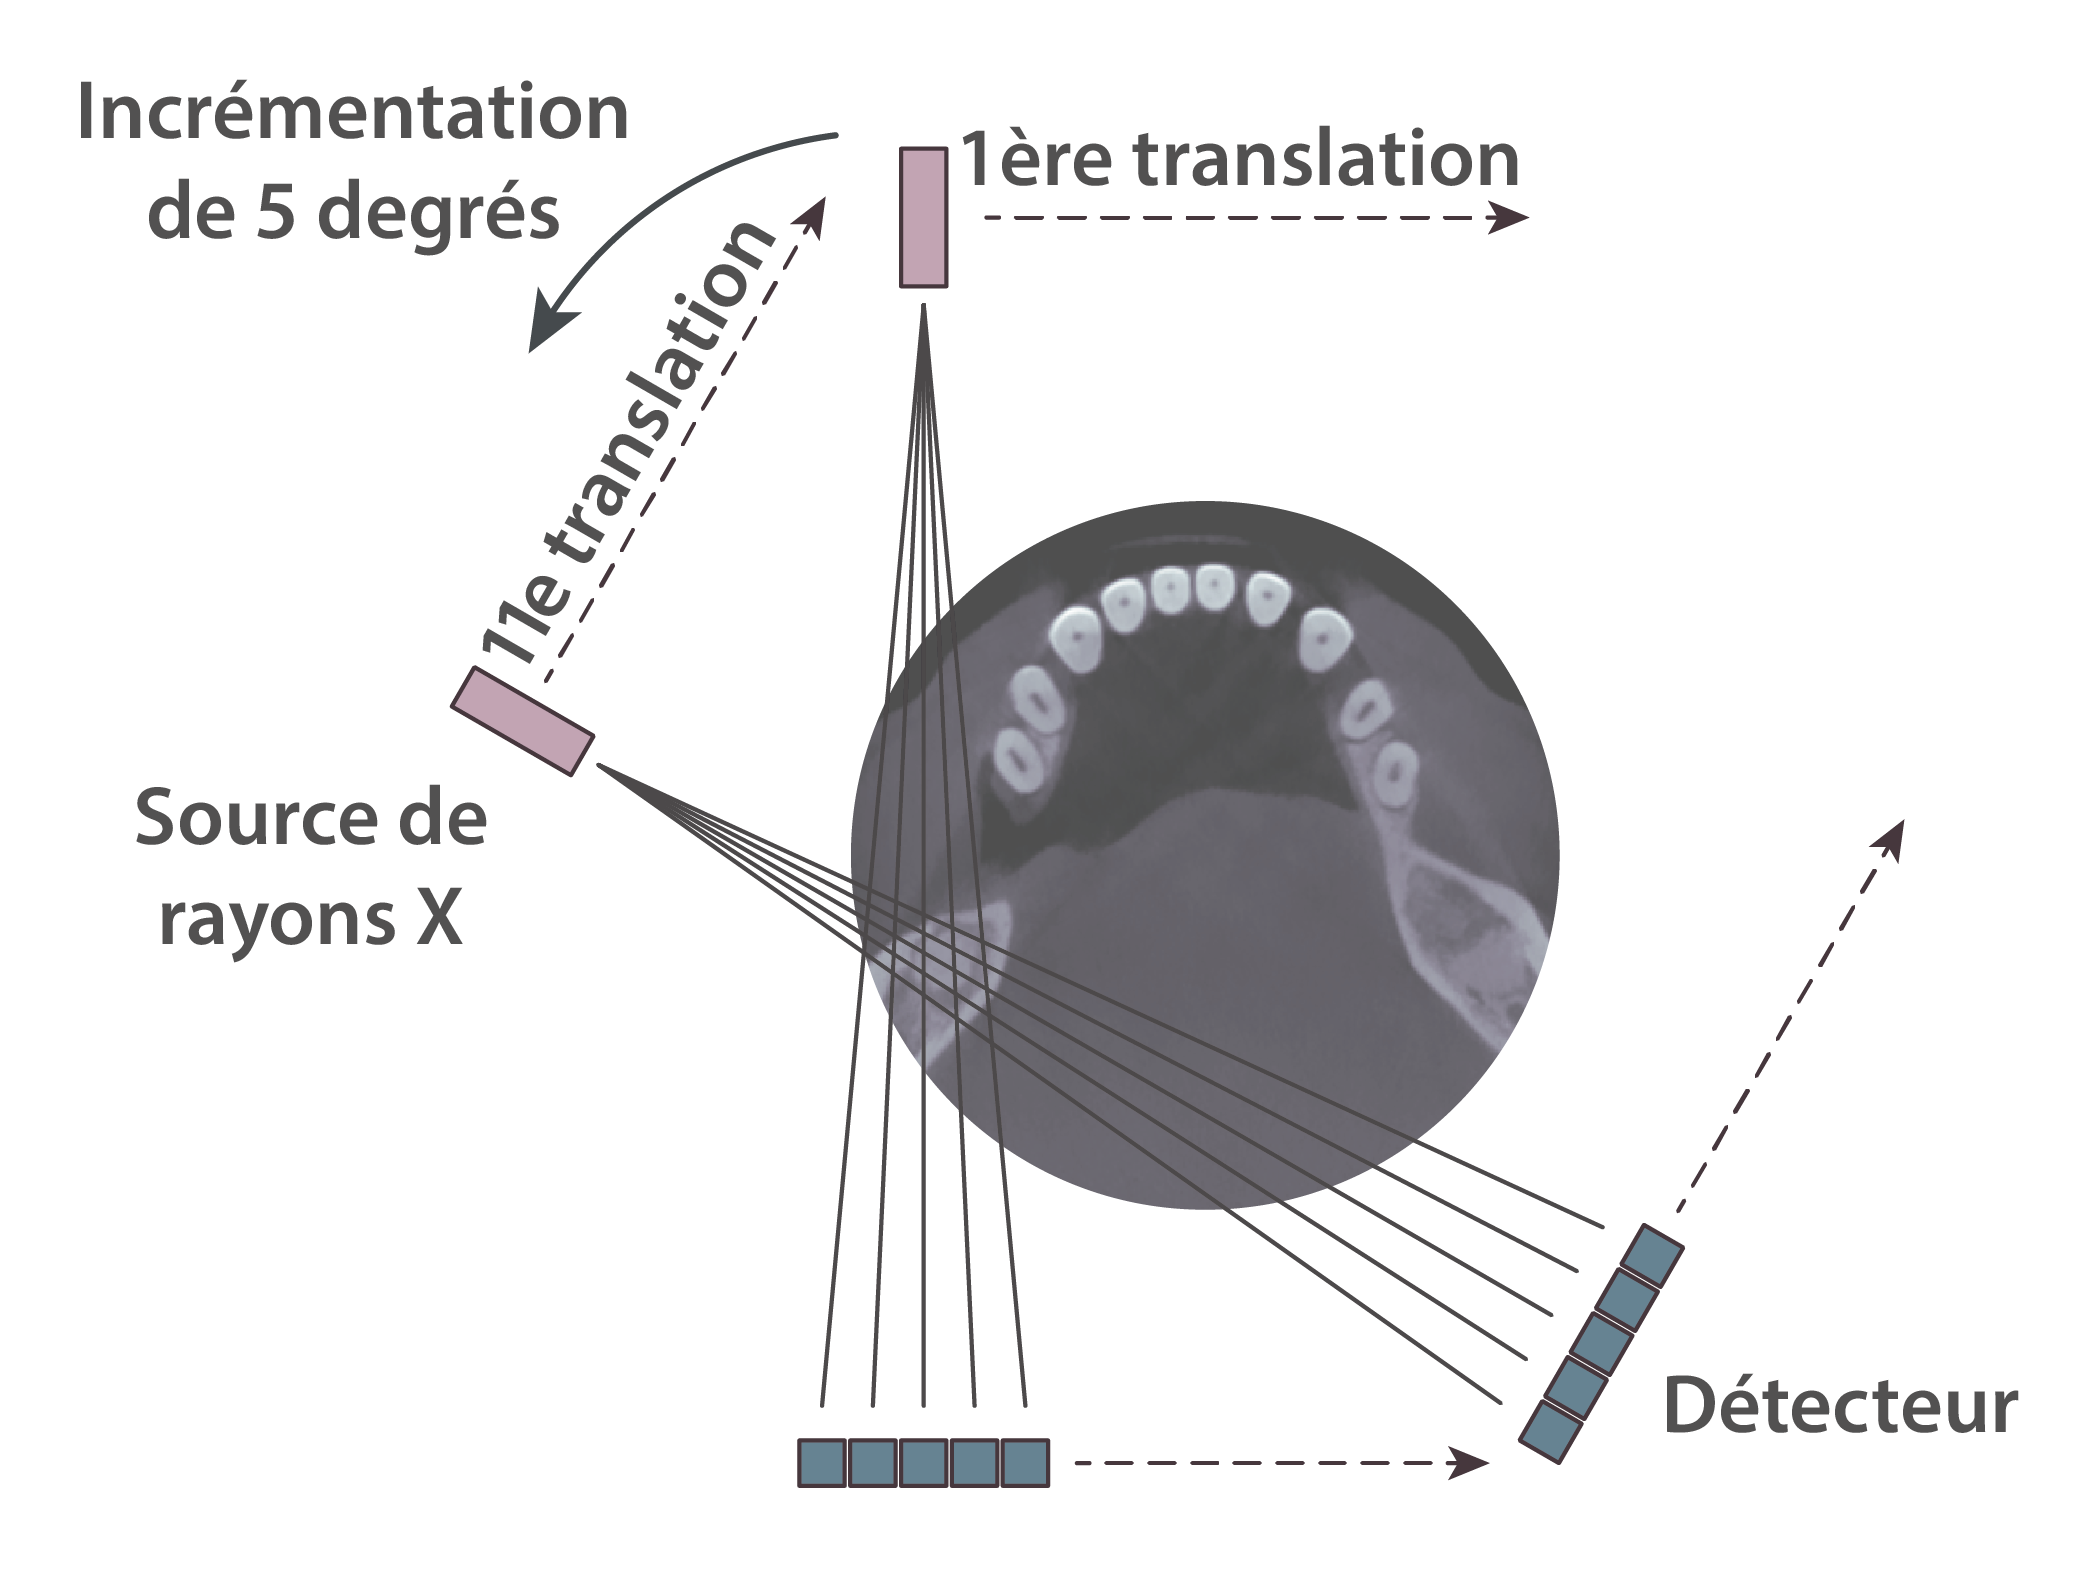
\includegraphics[height=5.5cm]{generation_Generation_2.png}
      \label{sub:gen2}
                         } \\
    \subfloat[$3^{\text{e}}$ génération]{
      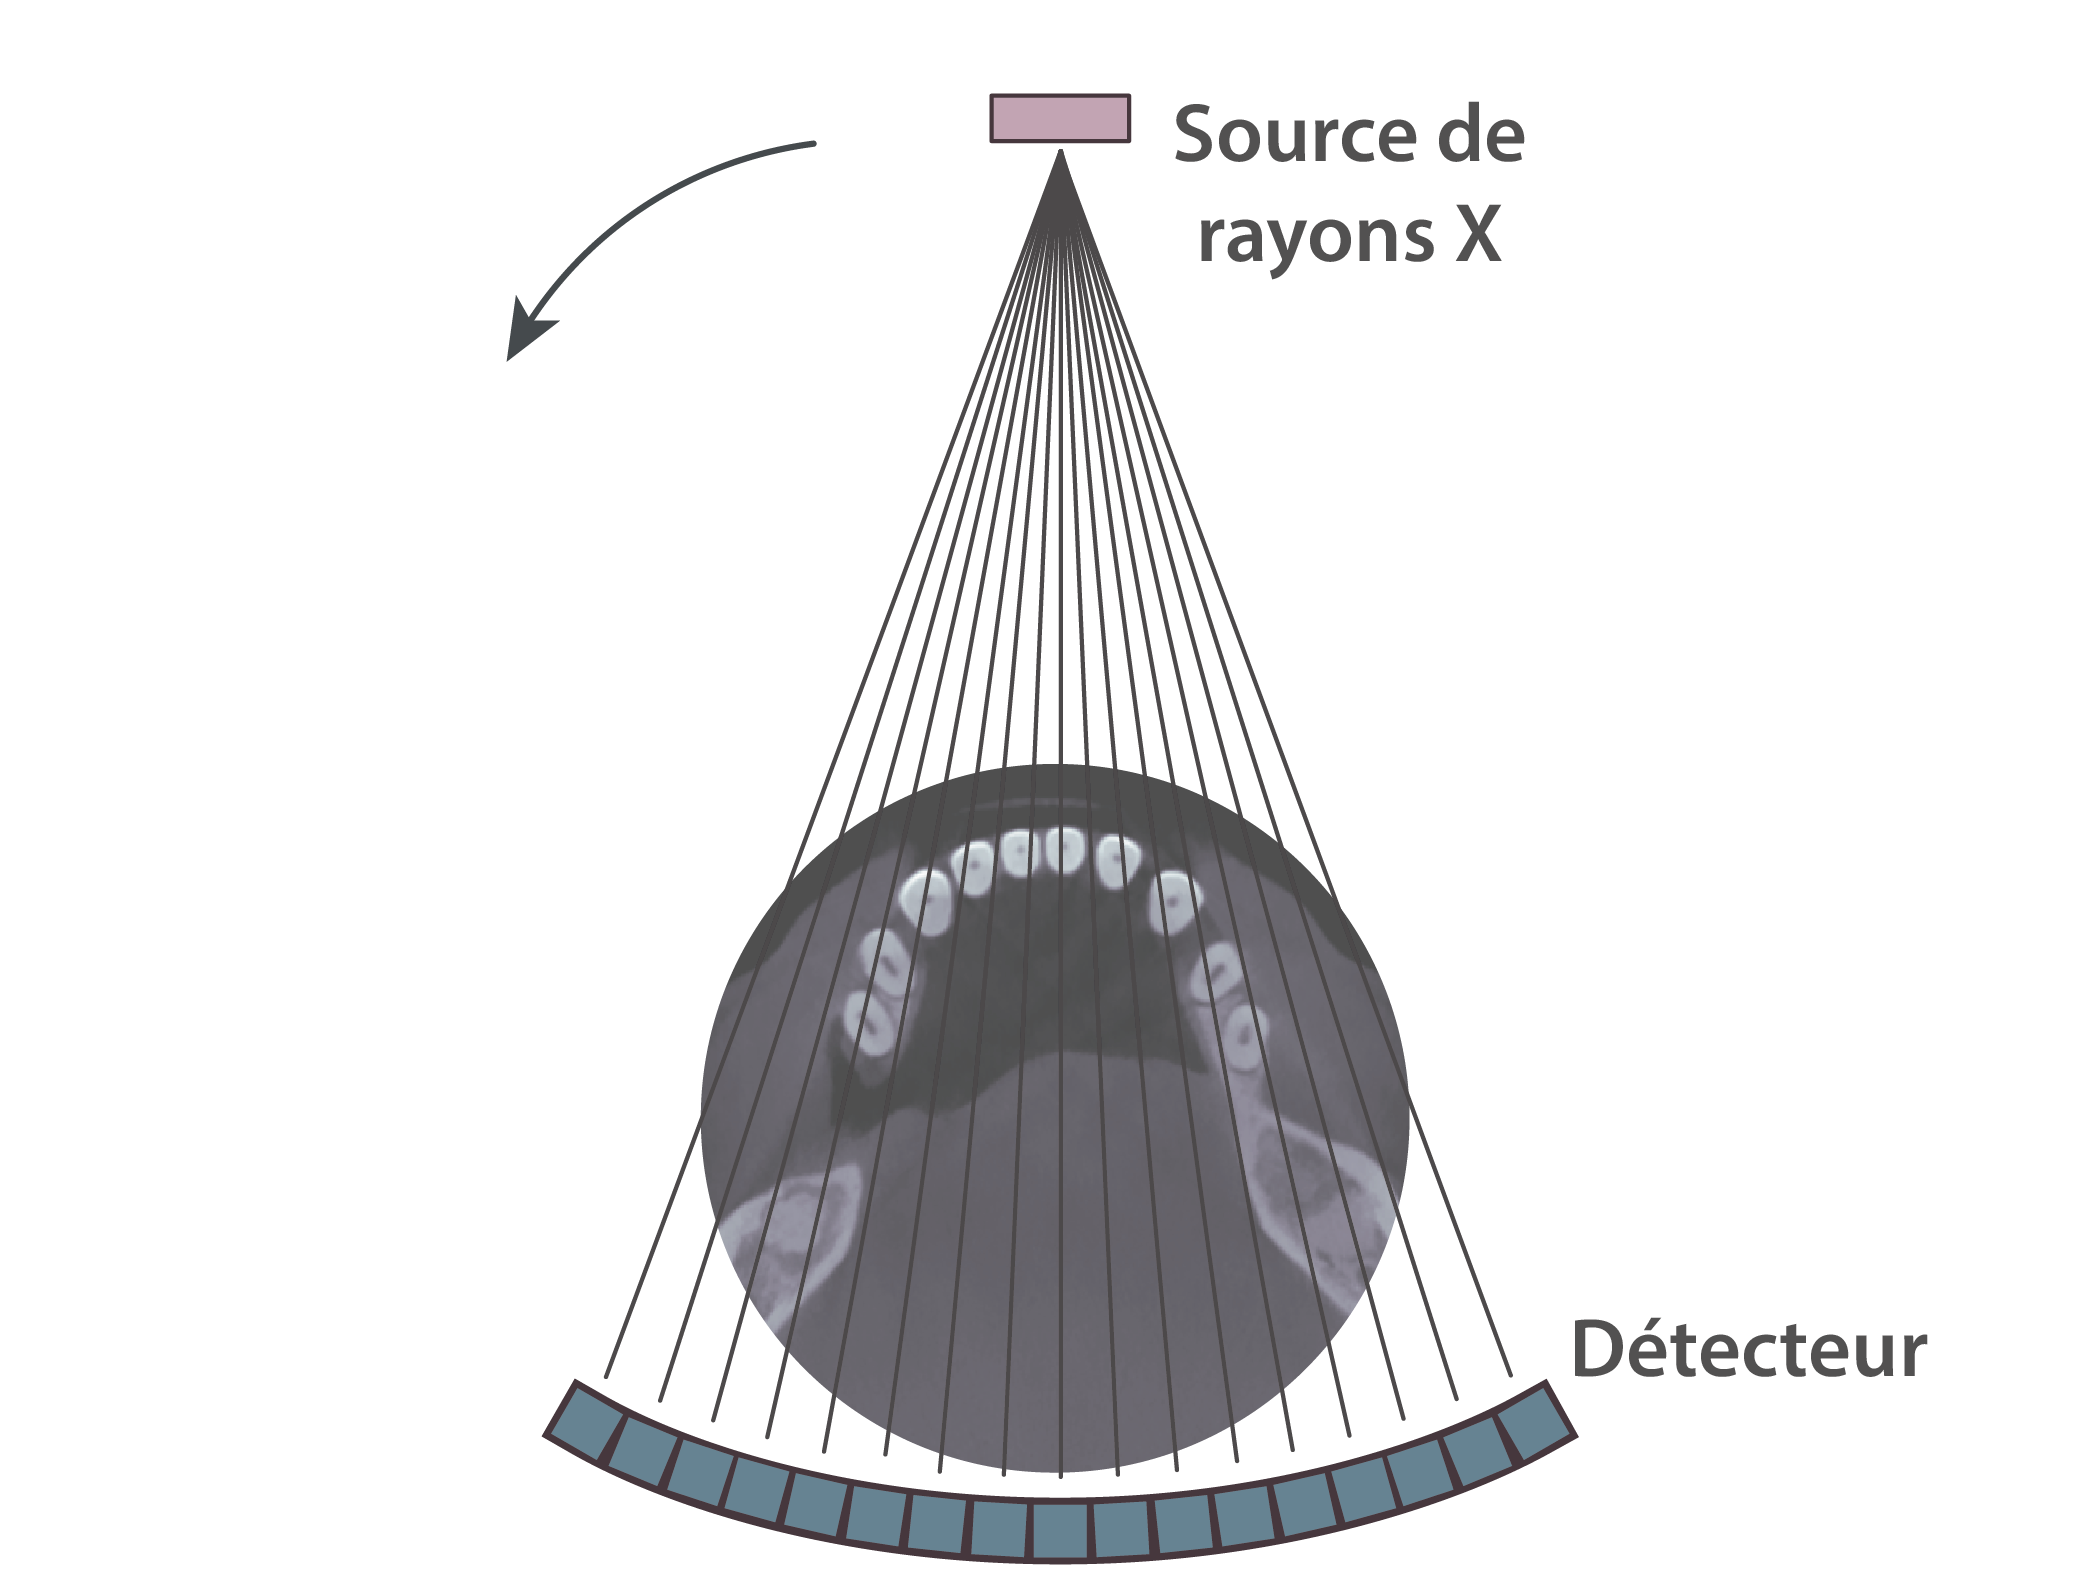
\includegraphics[height=5.5cm]{generation_Generation_3.png}
      \label{sub:gen3}
                         }
    \caption{Différentes générations de scanner.}
    \label{fig:scanner_gen}
  \end{center}
\end{figure} 

Pour la géométrie en éventail{\hypersetup{linkcolor=black}\footnote{\textit{fan beam} pour faisceau en éventail dans la littérature}}, la source est ponctuelle et le faisceau de rayons X a une forme d'éventail. Le détecteur est plat ou incurvé. On retrouve cette géométrie dans les scanners de seconde et troisième génération. Les scanners de seconde génération avaient pour principal but de réduire considérablement le temps d'acquisition par rapport à la première génération. Le faisceau de rayons X a une forme d'éventail et le détecteur multi-pixels permet de réduire le nombre d'angles d'acquisition (figure~\ref{sub:gen2}). Un scan pouvait être effectué en moins d'une minute avec cette génération de scanner. 
La troisième génération de scanner a vu disparaître la translation nécessaire pour chaque angle. Le détecteur est devenu suffisamment grand pour contenir l'intégralité de l'objet dans son champ de vue (figure~\ref{sub:gen3}). Ainsi, seule une rotation autour du patient était suffisante, ce qui a permis de réduire le temps d'acquisition en dessous de 3 secondes. 

Aujourd'hui, les détecteurs utilisés peuvent être plans ou incurvés, indépendamment de la forme du faisceau, et le scanner n'effectue qu'une seule rotation autour du patient, sans translation et en un temps très court. 

Les scanners présentés jusqu'à présent permettent de reconstruire une image 2D. Si l'on veut reconstruire un volume 3D du patient, on peut répéter plusieurs fois un scan 2D pour reconstruire plusieurs coupes qui formeront le volume 3D. Aujourd'hui, le couple source-détecteur suit une trajectoire hélicoïdale : ils tournent plusieurs fois autour du patient en effectuant une légère translation pour obtenir les mesures sur plusieurs coupes. Une dernière technique est d'utiliser un détecteur rectangulaire composé de plusieurs lignes de pixels. 

La géométrie conique{\hypersetup{linkcolor=black}\footnote{\textit{cone beam} dans la littérature}} utilise un faisceau en forme de cône. La source reste ponctuelle, mais plusieurs plans de faisceau en éventail sont collectés simultanément pour couvrir un volume. Cependant, la source étant ponctuelle, un seul plan est perpendiculaire à l'axe de rotation, les autres sont inclinés. Pour cette géométrie, l'acquisition se fait en n'effectuant qu'un seul tour autour du patient. Le processus de reconstruction tomographique est noté dans ce cas CBCT (\textit{Cone Beam Computed Tomography}). Les données obtenues en géométrie conique correspondent à des radiographies. 

Dans la suite de cette thèse, c'est cette dernière géométrie qui nous intéressera. Cependant, la formulation géométrique étant complexe, les premières explications sur la reconstruction tomographique resteront dans le cadre simplifié de la reconstruction 2D et de la géométrie parallèle. On retrouve les trois différentes géométries dans la figure~\ref{fig:diff_geometry}. 


\begin{figure}[H]
\centering
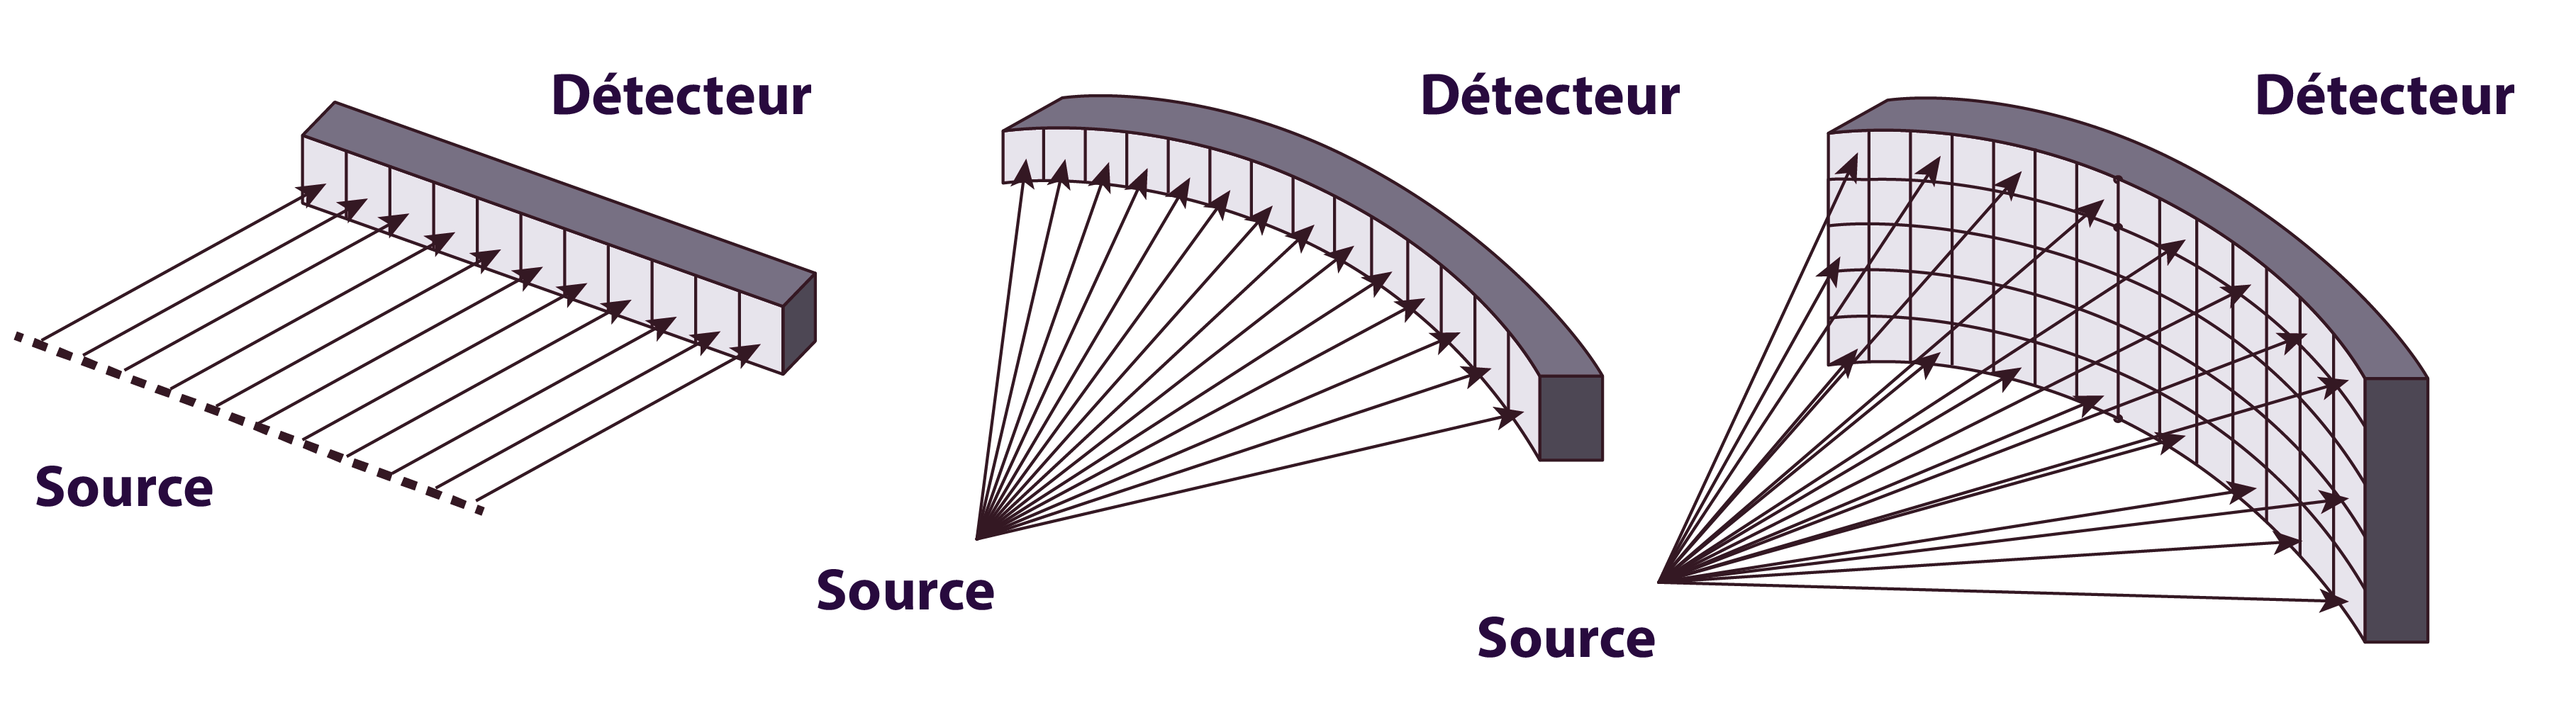
\includegraphics[width=\textwidth]{geometry-04.png}
\caption{Illustration des différentes géométries d'acquisition. De gauche à droite : parallèle, en éventail, conique.}
\label{fig:diff_geometry}
\end{figure}


%**************************************
\section{Applications en imagerie médicale}
%**************************************
	\label{sec:app_imagerie_medicale}

Les utilisations de la tomographie en imagerie médicale sont nombreuses. Puisqu'elle utilise la transmission des rayons X, on comprend qu'elle bénéficie des avantages de celle-ci et qu'elle sera utile pour observer les os et par exemple, détecter des fractures. Mais elle permet également de s'affranchir de la superposition des différents matériaux traversés sur la radiographie, et donc de déterminer leur position relative. Elle améliore aussi le contraste dans les tissus et des anomalies dans les poumons peuvent par exemple être détectées grâce à une image de scanner. Enfin, avec l'apparition des produits de contraste, elle trouve des applications en angiographie et peut imager les vaisseaux sanguins ou encore le cerveau. %Avec la tomographie par émission, on peut aussi détecter les tumeurs, déterminer leur position et leur taille et planifier les séances de radiothérapie. 

Nous allons, dans la suite de cette partie, parler plus précisément de la tomographie par faisceau conique (CBCT) et de ses applications en imagerie dentaire.


%------------------------------
\subsection{Système CBCT en imagerie dentaire}

\begin{figure}
\centering
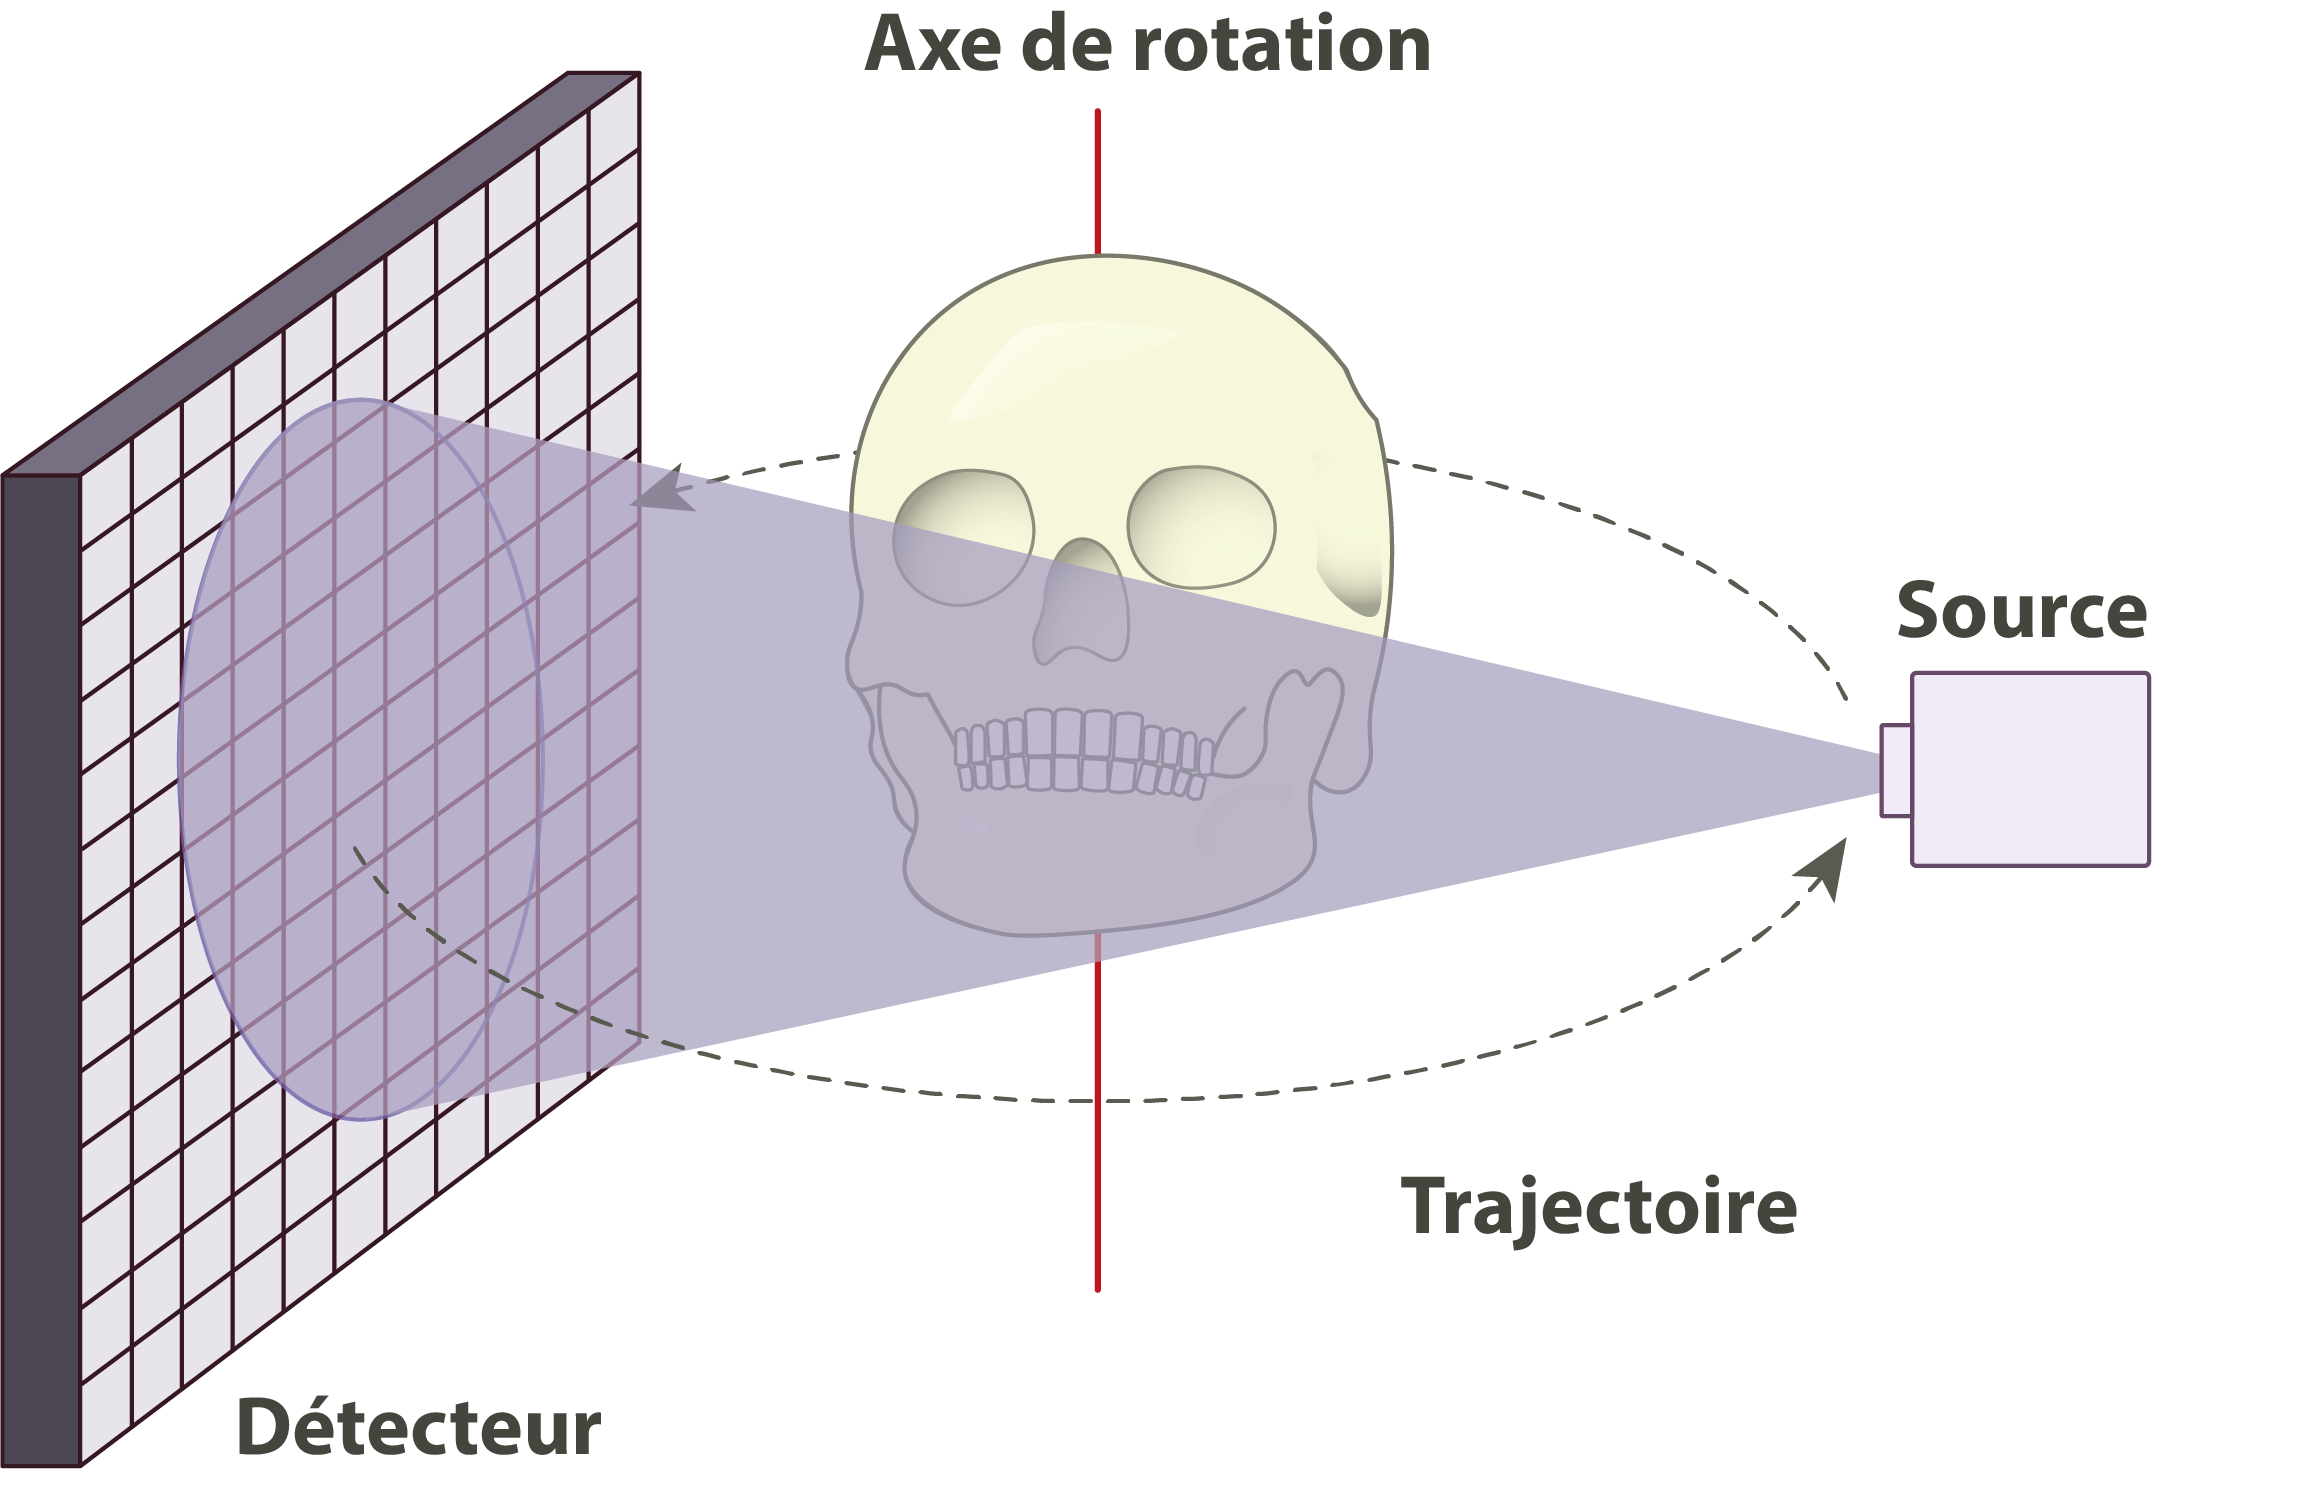
\includegraphics[width=0.7\textwidth]{geometry_cone_beam.png}
\caption{Schéma d'une acquisition CBCT.}
\label{fig:schema-cbct}
\end{figure}

Lors d'un examen de scanner CBCT, le patient est installé assis ou debout et garde sa tête immobile. La source de rayons X et le détecteur vont effectuer une rotation simultanée autour du patient et acquérir les images radiographiques nécessaires à la reconstruction. La figure~\ref{fig:schema-cbct} illustre le fonctionnement du CBCT et sa géométrie d'acquisition. Une fois les projections récupérées par l'ordinateur, elles sont pré-traitées avant qu'un algorithme de reconstruction n'effectue la reconstruction 3D. Les images obtenues peuvent ensuite subir encore quelques post-traitements, en particulier lors d'acquisition à faible dose ou de présence de métal, et sont finalement prêtes pour le diagnostic et/ou la modélisation 3D. 

Comparé aux scanners conventionnels, le CBCT offre plusieurs avantages. Il permet de diminuer la dose envoyée au patient tout en offrant une meilleure résolution spatiale grâce à ses petits voxels isotropiques \citepp{Grondin2013,Dartus2021}. Par la position assise ou debout du patient, les scanners CBCT sont de plus petite taille que les scanners conventionnels. Ils peuvent donc être installés dans les cabinets dentaires. Ils sont également beaucoup moins coûteux, ce qui les rend facilement accessibles pour les dentistes qui exercent dans des cabinets en dehors d'un milieu hospitalier. 


%--------------------------------
\subsection{En imagerie dentaire}

En imagerie dentaire, les scanners CBCT sont utilisés pour produire des images 3D des structures dentaires, des tissus mous, des canaux contenant les nerfs et des os présents dans la région maxillo-faciale. Ils fournissent des images détaillées de l'os et permettent de détecter des anomalies dans cette région : la denture, les structures osseuses du visage, la cavité nasale et les sinus. Nous retrouvons dans la figure~\ref{fig:schema_dent} un schéma d'une dent avec les différentes structures anatomiques importantes. 

Les points importants à examiner dans un scanner de la mâchoire sont : 
\begin{itemize}[label=$\blacklozenge$]
	\item la zone ligamentaire autour des dents
	\item l'os alvéolaire, pour la pose d'implant
	\item les potentielles lésions autour des racines des dents
	\item les canaux à l'intérieur des dents, leur longueur et leur largeur 
	\item la position du canal mandibulaire, particulièrement importante pour ne pas avoir de contact avec le nerf à l'intérieur pendant une intervention chirurgicale. 
\end{itemize}

\begin{figure}
	\centering
	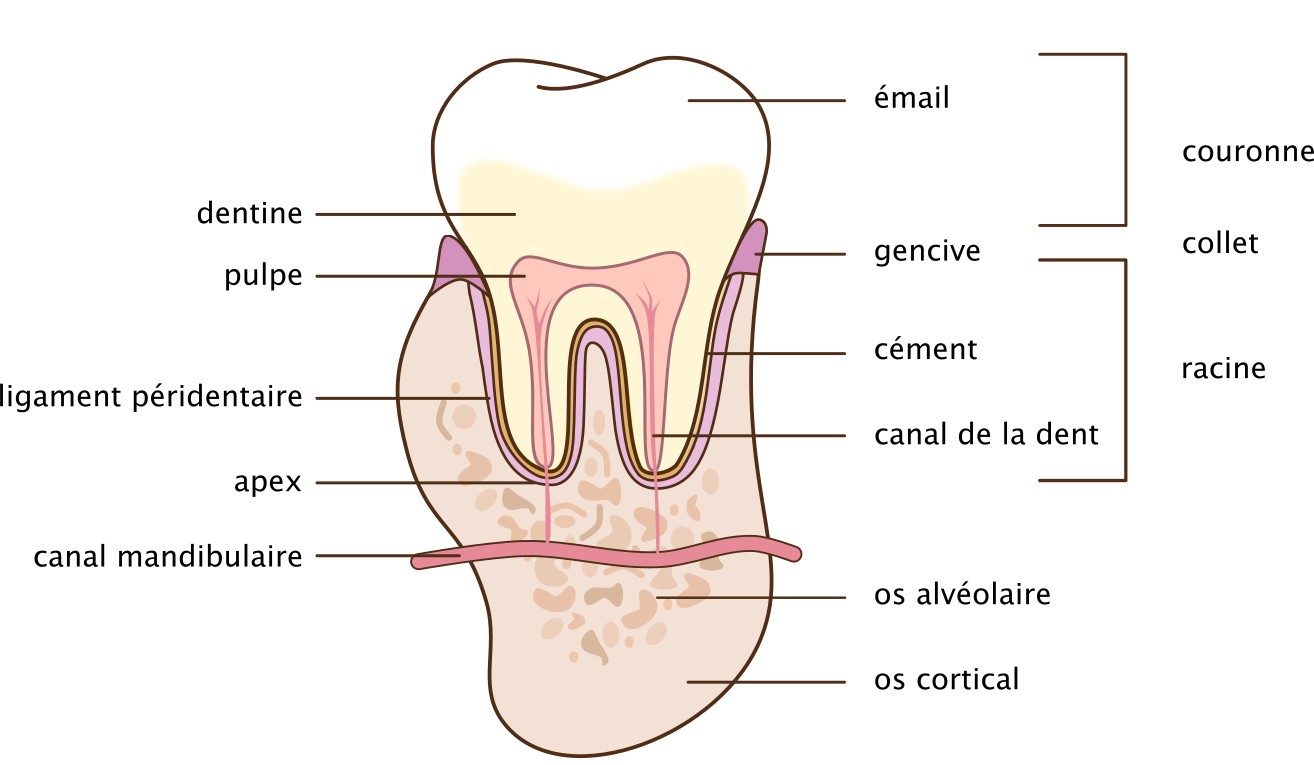
\includegraphics[width=0.7\textwidth]{dents.png}
	\caption{Schéma d'une dent.}
	\label{fig:schema_dent}
\end{figure}

La tomographie en imagerie dentaire est une modalité d'imagerie particulièrement difficile, les structures importantes recherchées par le praticien sont souvent très fines et nécessitent une excellente qualité de reconstruction. Cependant, de nombreux facteurs physiques dégradent la qualité de l'image. La position assise du patient le rend moins stable que lorsqu'il est allongé, et ses mouvements lors de l'acquisition créent des artefacts dans l'image reconstruite s'ils ne sont pas corrigés. De plus, la zone maxillo-faciale contient souvent du métal (implants, bagues orthodontiques, etc.) à l'origine d'artefacts métalliques dans les images. Le métal absorbant bien plus les rayons X que les os ou les tissus mous, les projections manquent d'informations pour représenter correctement le volume à reconstruire.

De part son aspect cancérigène, il est nécessaire de réduire la dose au maximum afin de limiter les risques pour le patient. Cependant, en diminuant la dose envoyée, l'importance relative du  bruit statistique naturellement présent dans les acquisitions augmente et le rapport signal sur bruit{\hypersetup{linkcolor=black}\footnote{SNR pour \textit{Signal to Noise Ratio}}} diminue, la qualité de la reconstruction est alors dégradée. 
En imagerie de la mâchoire, afin de ne pas irradier le patient avec des rayons inutiles, le scanner envoie des rayons seulement dans la région d'intérêt qui est souvent plus petite que la taille de la tête du patient. On obtient alors ce que l'on appelle des projections tronquées, qui ne contiennent pas l'intégralité de l'objet sur chaque angle, et qui génèrent des incohérences lors du processus de reconstruction. Les différents artefacts, ainsi que leurs causes et leurs conséquences, seront détaillés dans le chapitre \ref{chap:2}.


%*************
\section*{}
%*************

Dans ce premier chapitre, nous avons expliqué comment les rayons X sont produits et comment ils interagissent avec la matière pour donner les images de radiographie utilisées en imagerie médicale. Grâce aux propriétés d'absorption propres à chacun des matériaux, il est possible de distinguer les différents matériaux qui composent l'intérieur d'un objet ou d'un patient, sans intervention chirurgicale. 

La tomographie à rayons X utilise des données d'atténuation, aussi appelées projections, de l'objet considéré pour reconstruire des images en coupe de celui-ci. Cela permet de séparer des structures qui se superposent dans une radiographie. C'est une technique d'imagerie utilisée dans divers domaines, mais dont les applications sont surtout connues du grand public en imagerie médicale. 

En imagerie dentaire, les scanners CBCT ont permis de rendre accessible la tomographie 3D à un grand nombre de praticiens. Elle est utilisée dans de nombreuses interventions et domaines : odontologie, parodontie, chirurgie, implantologie, orthodontie ou encore pédodontie.  

Le prochain chapitre traitera de la partie reconstruction, de ses bases mathématiques et des premiers algorithmes qui ont été utilisés.

\vfill

\bibliographystyle{apalike-fr}
\bibliography{bib}

